\chapter{轴突的生长和引导} \label{chap:chap47}


在前两章中,我们看到了神经元是如何在正确的时间和正确的位置以适当的数量生成的。
这些早期发育步骤为后来的事件奠定了基础,这些事件指导神经元与目标细胞形成功能性联系。
为了形成连接,神经元必须延伸较长的过程——轴突和树突——它们允许与突触后细胞连接以及来自其他神经元的突触输入。
在本章中,我们将研究神经元如何精心制作轴突和树突,以及轴突如何被引导至它们的目标。


我们通过讨论某些神经元过程如何变成轴突和其他树突来开始本章。
然后我们描述了生长中的轴突,它可能必须经过很长的距离并忽略许多不合适的神经元伙伴,然后才能在正确的区域终止并识别其正确的突触目标。
我们考虑轴突克服这些挑战的策略。
最后,我们通过描述两个经过充分研究的轴突通路的发展来说明轴突引导的一般特征:
一个将视觉信息从视网膜传递到大脑,另一个将皮肤感觉信息从脊髓传递到大脑。



\section{轴突和树突之间的差异在发育早期就出现了}

神经元的过程在长度、厚度、分支模式和分子结构方面差异很大。
尽管如此,大多数神经元过程都属于两个功能类别之一:轴突和树突。
一个多世纪以前,圣地亚哥·拉蒙·卡哈尔 (Santiago Ramón y Cajal) 假设这种区别是神经元向特定方向传输信息的能力的基础,他将这一想法形式化为动态极化定律。
卡哈尔写道,“神经冲动的传递总是从树突分支和细胞体到轴突。” 在电生理学方法能够胜任这项任务之前的几十年里,这条定律提供了一种从组织学上分析神经回路的方法。
尽管发现了例外情况,但 Ramón y Cajal 定律仍然是将结构与神经系统功能联系起来的基本原理,并强调了了解神经元如何获得极化形式的重要性。


理解神经元极化如何发生的进展在很大程度上来自对取自啮齿动物大脑并在组织培养中生长的神经元的研究。
孤立生长的海马神经元发展过程让人联想到在体内看到的过程:一个单一的、长的、圆柱形的轴突和几个较短的、锥形的树突(图 \ref{fig:47_1}A)。
由于细胞骨架和突触蛋白以不同方式靶向这些成分,因此轴突和树突获得了独特的分子特征。
例如,一种特定形式的 Tau 蛋白位于轴突中,MAP2 蛋白位于树突中(图 \ref{fig:47_1}B)。


\begin{figure}[htbp]
	\centering
	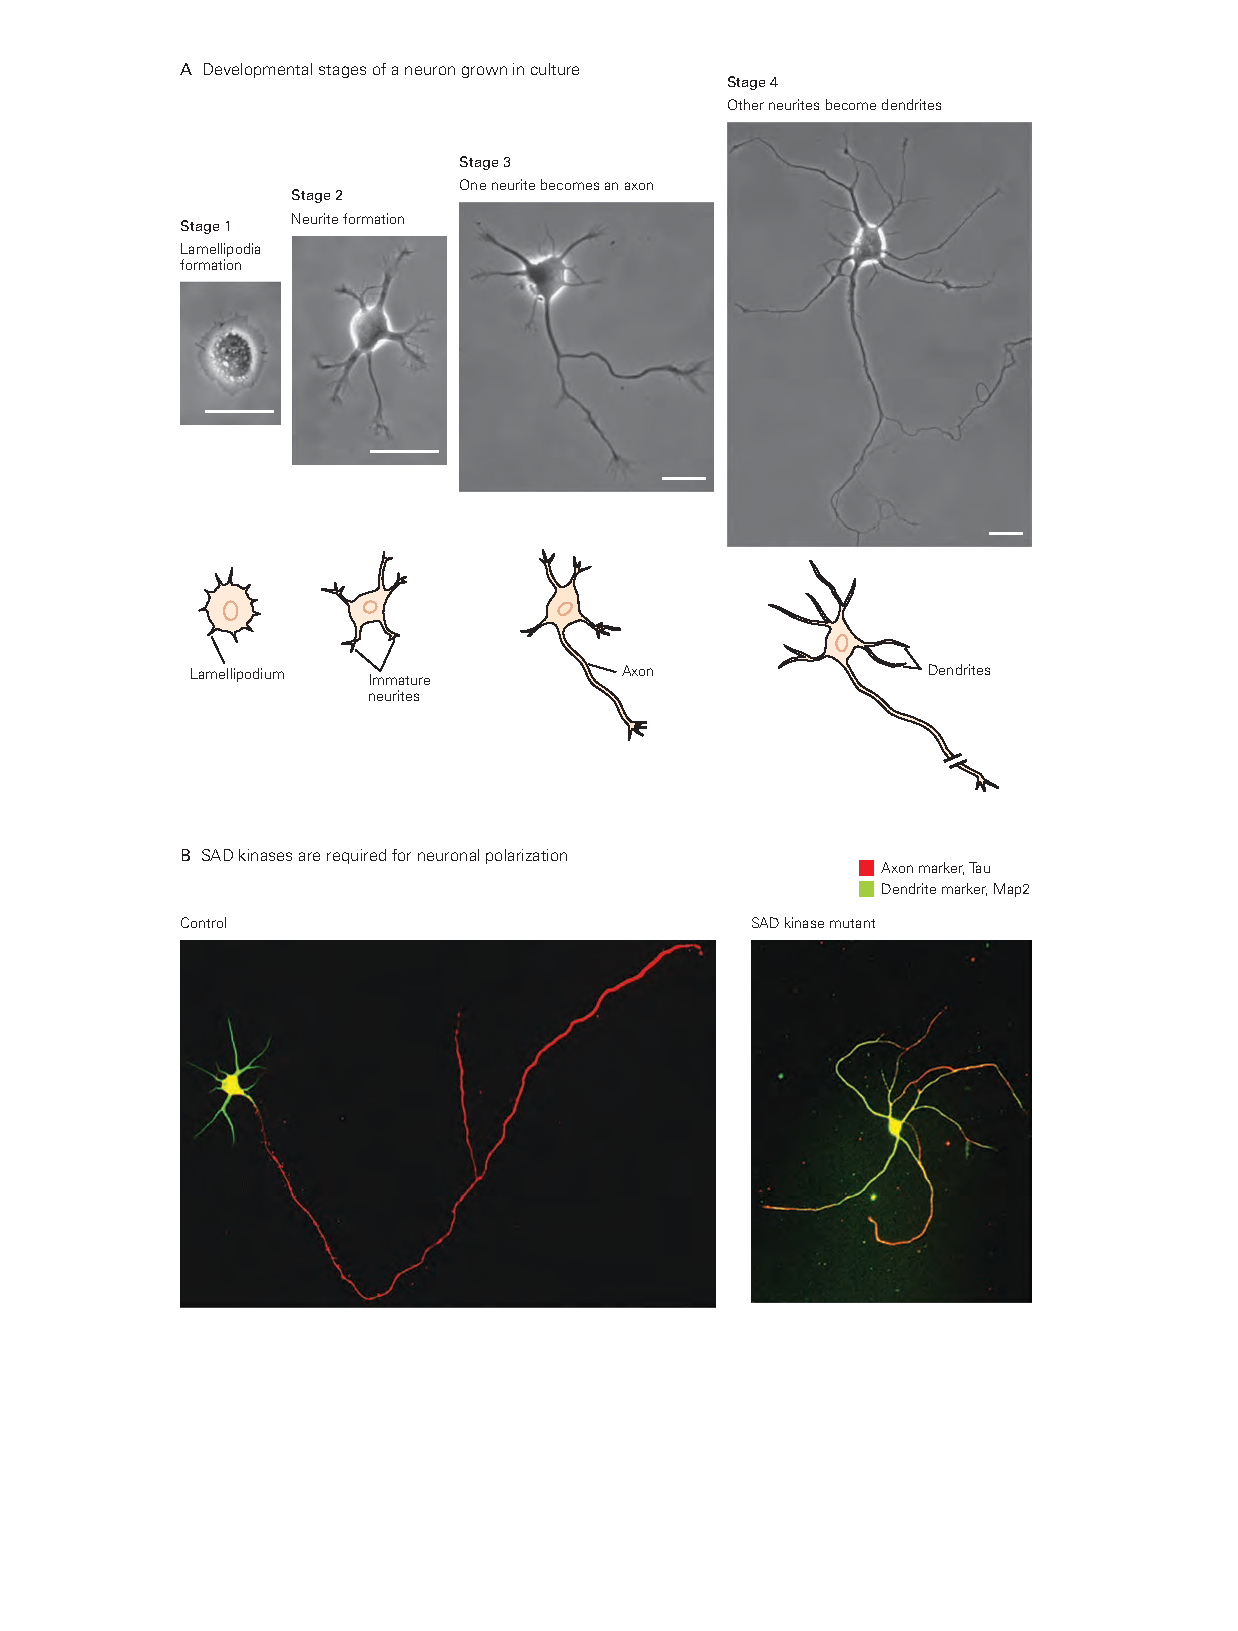
\includegraphics[width=0.75\linewidth]{chap47/fig_47_1}
	\caption{轴突和树突的分化标志着神经元极性的出现。 A. 在组织培养中生长的海马神经元极化的四个阶段。 (经许可改编自 Kaech 和 Banker 2006。版权所有 © 2007 Springer Nature。) B. 在培养物中生长的海马神经元具有多个短而粗的树突,这些树突富含微管相关蛋白 MAP2。 它们还拥有一个长轴突,其特征是微管相关蛋白 tau 的去磷酸化形式(左)。 从突变小鼠中分离出的培养神经元缺乏 Par 家族基因(SAD 激酶)的表达。 神经元生成的神经突同时表达 tau 和 MAP2,分别是轴突和树突的标记。 这些神经突的长度和直径介于轴突和树突之间(右)。 (经许可转载自 Kishi 等人,2005 年。)}
	\label{fig:47_1}
\end{figure}


培养的神经元对于发育研究特别有用,因为它们最初没有显示出明显的极化迹象,并在固定的细胞步骤序列中逐渐获得它们的专门特征。
这个序列从几个短流程的扩展开始,每个流程都等同于其他流程。
此后不久,一个过程被建立为轴突,其余过程获得树突特征(图 \ref{fig:47_1}A)。


这是怎么发生的?
维持细长过程和驱动生长的细胞骨架蛋白是这一过程的核心。
如果早期神经突中的肌动蛋白丝不稳定,细胞骨架就会重新配置,使神经突变成轴突;
其次,剩余的神经突反应成为树突。
如果新生的轴突被移除,剩余的轴突之一会迅速呈现出轴突特征。
该序列表明轴突规范是神经元极化中的关键事件,并且来自新形成的轴突的信号既抑制额外轴突的产生又促进树突形成。


抑制其他轴突的轴突衍生信号的性质尚不清楚,但对控制细胞骨架排列的信号的一些了解来自对一组由 Par 复合体基因编码的蛋白质的研究。
正如线虫蠕虫秀丽隐杆线虫中首次显示的那样,Par 蛋白参与细胞骨架重组的各个方面,包括神经元过程的极化。
缺乏 Par3、Par4、Par6 或 Par1 亲缘关系的哺乳动物前脑神经元会长出多个长度介于轴突和树突之间的突起,并带有两个突起的标记(图 \ref{fig:47_1}B)。


尽管在培养物中生长的神经元与大脑中的神经元相似,但它们被剥夺了关键的外在线索和信号。
培养的神经元彼此随机排列,而在发育中的大脑的许多区域,神经元排成一排,它们的树突指向同一方向(图 \ref{fig:47_2}A)。
随着神经元迁移到它们的目的地(第 \ref{chap:chap46} 章),轴突和树突通常分别作为它们的尾部和前导过程的延伸而生长。
这种体内和体外的差异意味着外在信号调节极化机制。 在发育中的大脑中,信号素和其他轴突引导因子的局部释放(本章后面将讨论)可能有助于树突的定向(图 \ref{fig:47_2}C)。
Par 蛋白复合物的作用是将这些细胞外信号与重新排列细胞骨架的细胞机制联系起来,这一过程部分是通过调节改变肌动蛋白或微管蛋白功能的蛋白质来实现的。
事实上,轴突中的 Tau 蛋白和树突中的 MAP2 蛋白都与微管相关并影响微管。
细胞骨架的差异也有助于其他机制放大轴突和树突之间的区别,例如分子的极化运输和轴突中专门的初始片段的产生。


\begin{figure}[htbp]
	\centering
	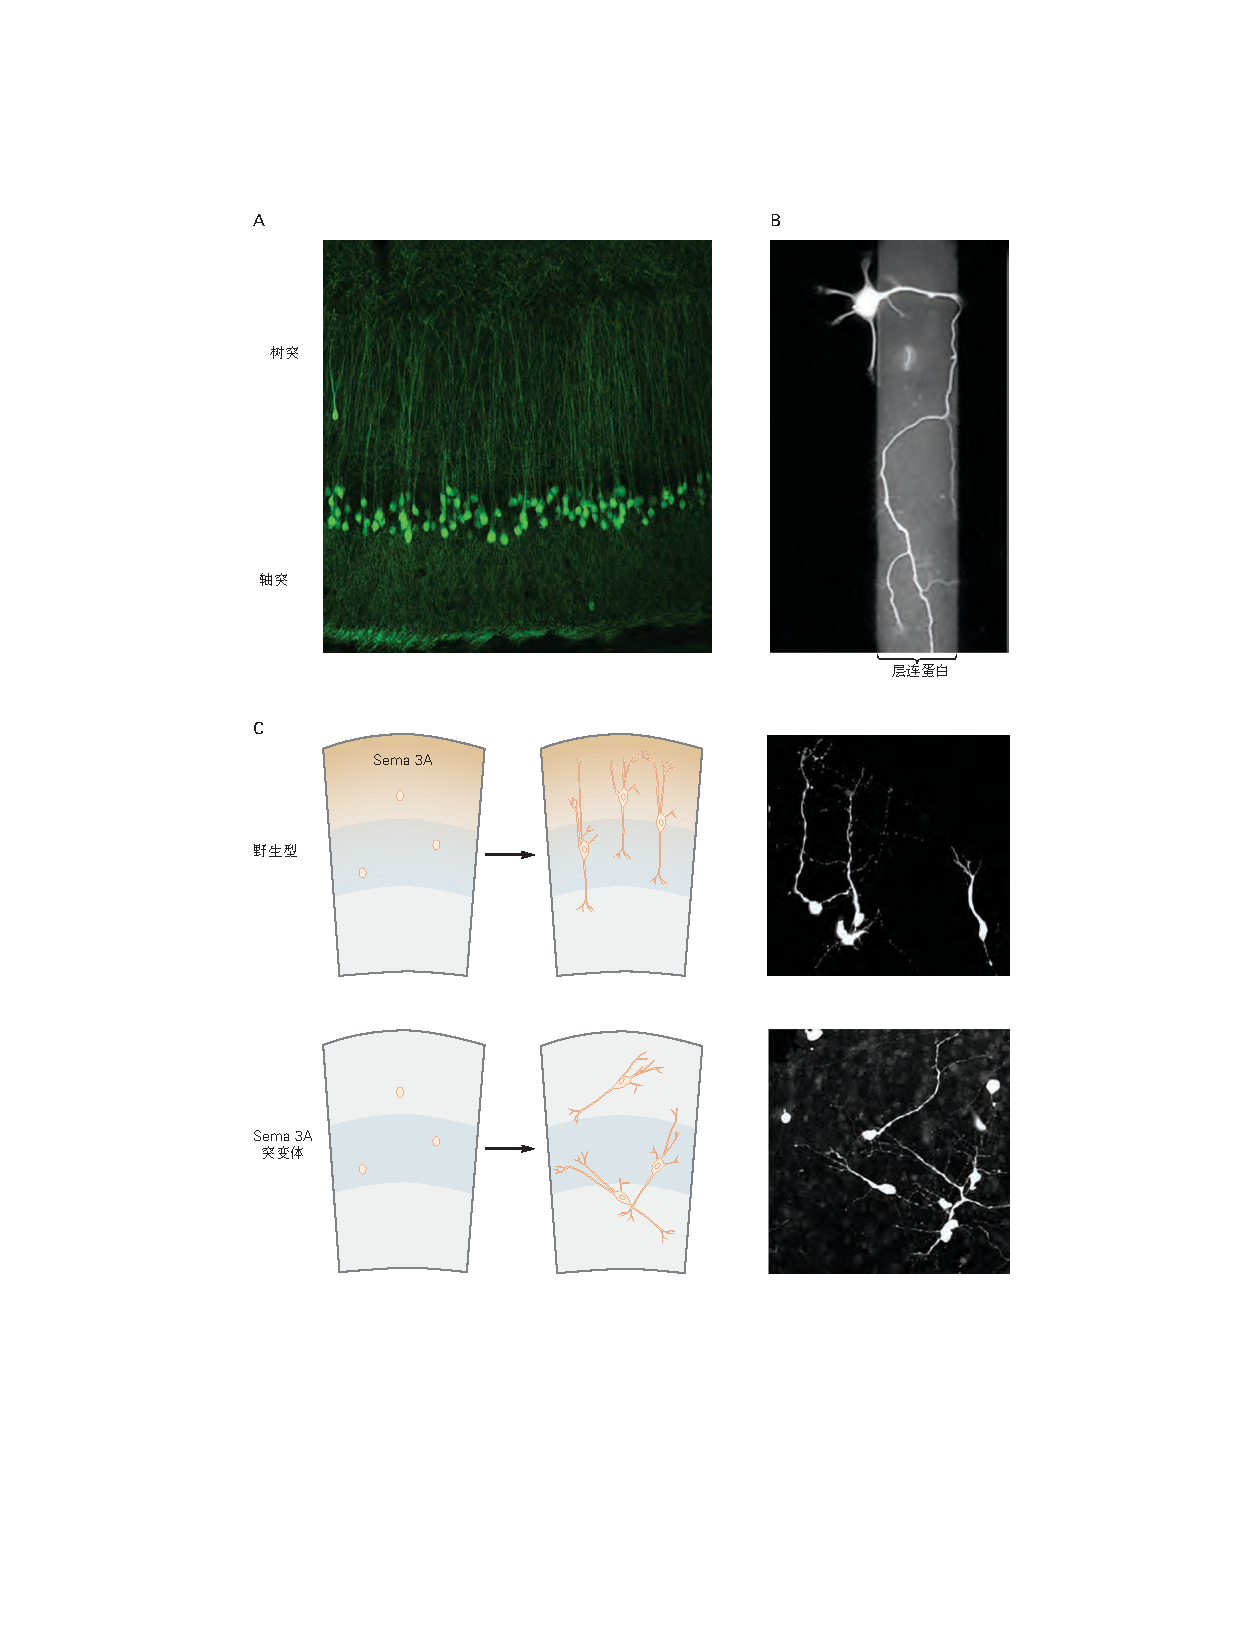
\includegraphics[width=0.65\linewidth]{chap47/fig_47_2}
	\caption{细胞外因素决定神经元过程是否变成轴突或树突。 A. 体内皮质锥体神经元显示出共同的轴突和树突方向。 B. 在层粘连蛋白上生长的神经元获得极性。 当皮质神经元将一个过程从不太吸引人的底物延伸到层粘连蛋白上时,该过程生长得更快,通常会变成轴突。 (图像经 Paul Letourneau 许可转载。)C. 在发育中的新皮质中,semaphorin-3A (Sema 3A) 由软脑膜表面附近的细胞分泌。 Semaphorin-3A 是树突生长的引诱剂,有助于建立神经元极性和方向。 在缺乏功能性 semaphorin-3A 的突变小鼠中,皮质锥体神经元的平行方向被破坏。 (经许可转载自 Polleux、Morrow 和 Ghosh 2000。版权所有 © 2000 Springer Nature。)}
	\label{fig:47_2}
\end{figure}


如果需要局部信号来极化大脑中的神经元,那么如何在组织培养的统一环境中建立极性?
一种可能的解释是,神经元内信号强度的微小变化,或来自其直接环境的信号的微小变化,将激活神经元一个小区域中的 Par 蛋白,触发最近的细胞突起成为轴突。
如果偶然,一个过程比它的邻居生长得稍微快一点,或者遇到一个加速神经突延伸的环境(图 \ref{fig:47_2}B),它成为轴突的机会显着增加。
据推测,这种原轴突过程发出的信号会降低其他过程效仿的机会,迫使它们变成树突。



\section{树突由内在和外在因素组成}

一旦发生极化,树突就会生长和成熟,获得将它们与轴突区分开来的结构特征。
新生树突形成分枝乔木,其分枝通常比轴突的分枝更多,更靠近细胞体。
此外,称为棘的小突起从许多树突的远端分支延伸。
最后,一些树突状分枝被缩回或“修剪”,使乔木具有最终和确定的形状(图 \ref{fig:47_3})。


\begin{figure}[htbp]
	\centering
	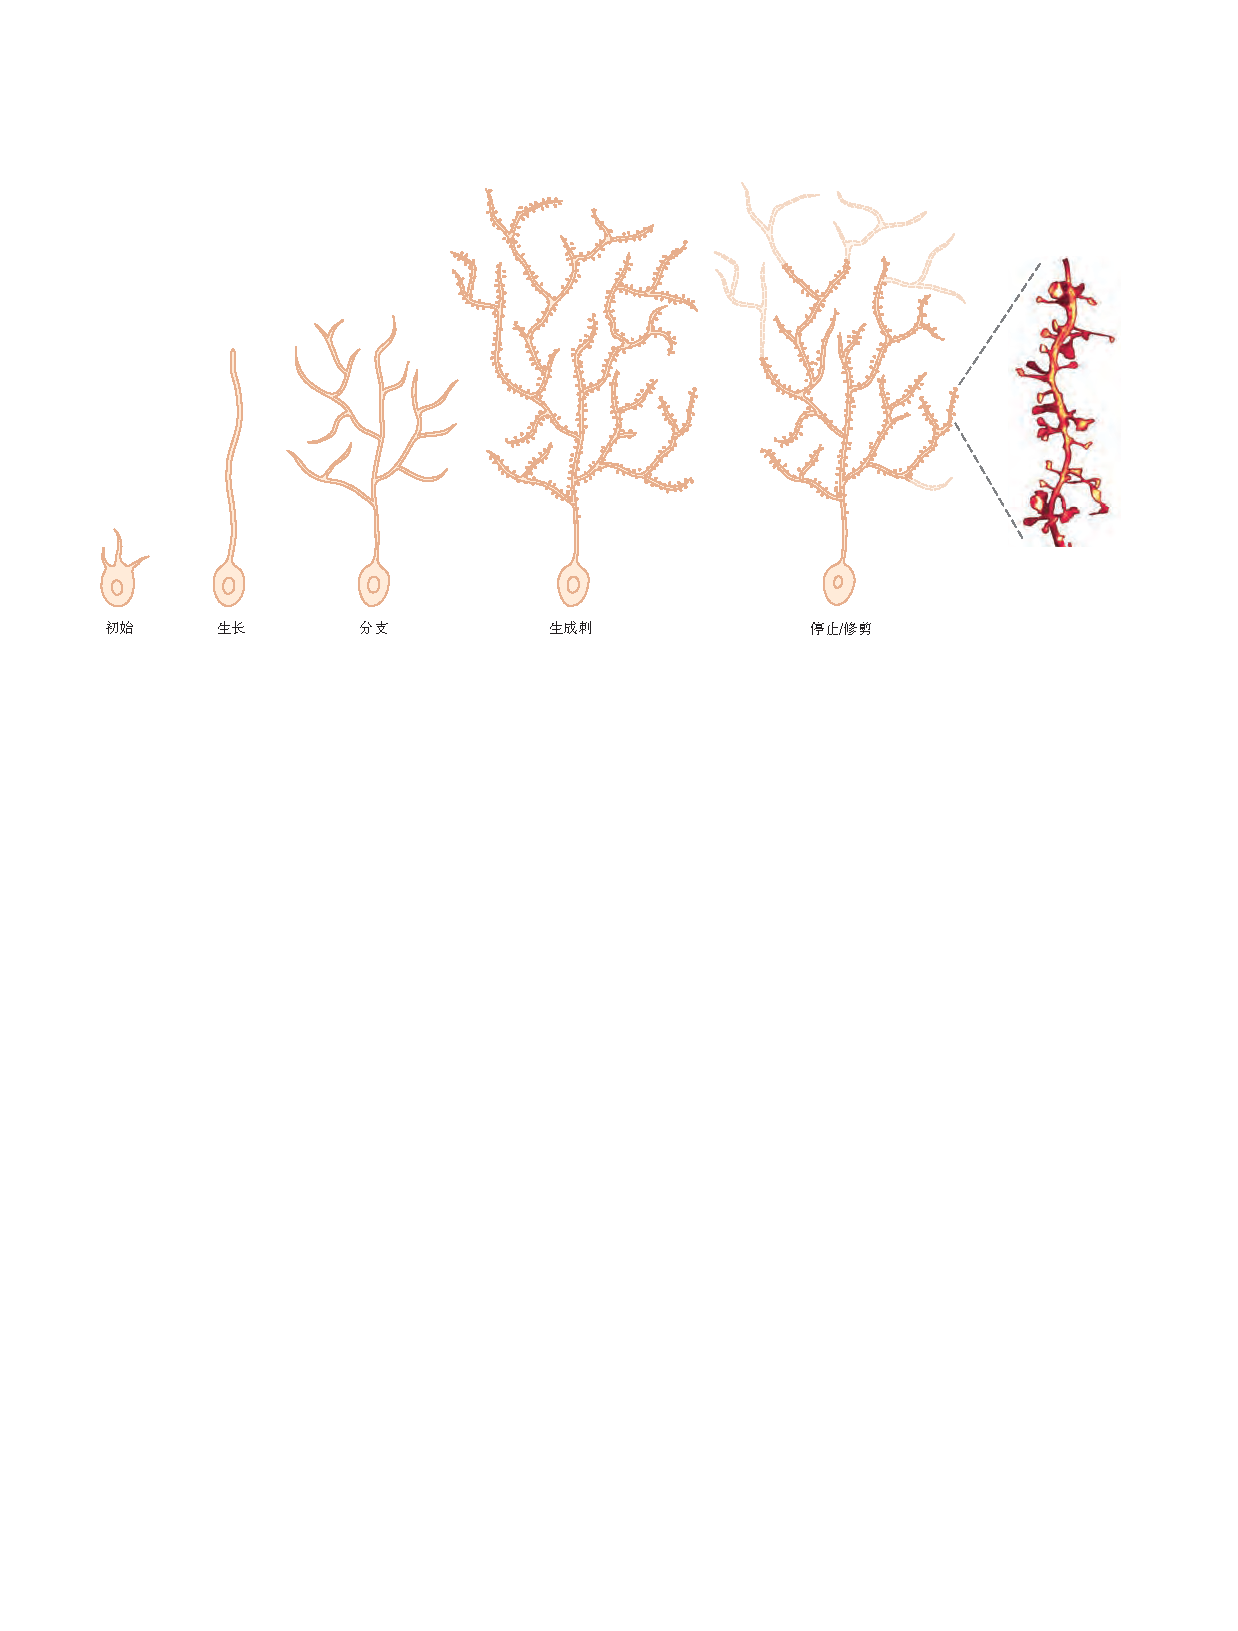
\includegraphics[width=0.95\linewidth]{chap47/fig_47_3}
	\caption{树突状分枝按一系列步骤发展。 树突的生长涉及精细分枝的形成,从中长出刺。 某些分支和刺后来被修剪以实现树突树枝化的成熟模式。 (右图的脊柱图片经许可转载自 Stefan W. Hell。)}
	\label{fig:47_3}
\end{figure}


尽管树突形成的核心特征对于许多神经元来说是共同的,但它们在神经元类型之间的数量、形状和分支模式方面存在显着差异。事实上,树突状乔木的形状是神经元分类的主要方式之一。
只需观察树突的模式,即可将小脑浦肯野细胞与颗粒细胞、脊髓运动神经元和海马锥体神经元区分开来。
这些变化对于不同神经元类型的不同功能至关重要。
例如,树突状乔木的大小及其分支的密度是其接收的突触数量的主要决定因素。


树枝状模式是如何建立的?
神经元必须具有关于其形状的内在信息,因为组织培养中的模式与体内的模式惊人地相似(图 \ref{fig:47_4})。
指定神经元亚型的转录程序(第 \ref{chap:chap46} 章)大概也编码有关神经元形状的信息。
在无脊椎动物和脊椎动物中,一些转录因子由特定的神经元类型选择性地表达,并且似乎致力于控制其树突状乔木的大小、形状和复杂性。
他们通过协调下游基因的表达来做到这一点,包括那些编码细胞骨架装置成分的基因和介导与邻近细胞相互作用的膜蛋白。


\begin{figure}[htbp]
	\centering
	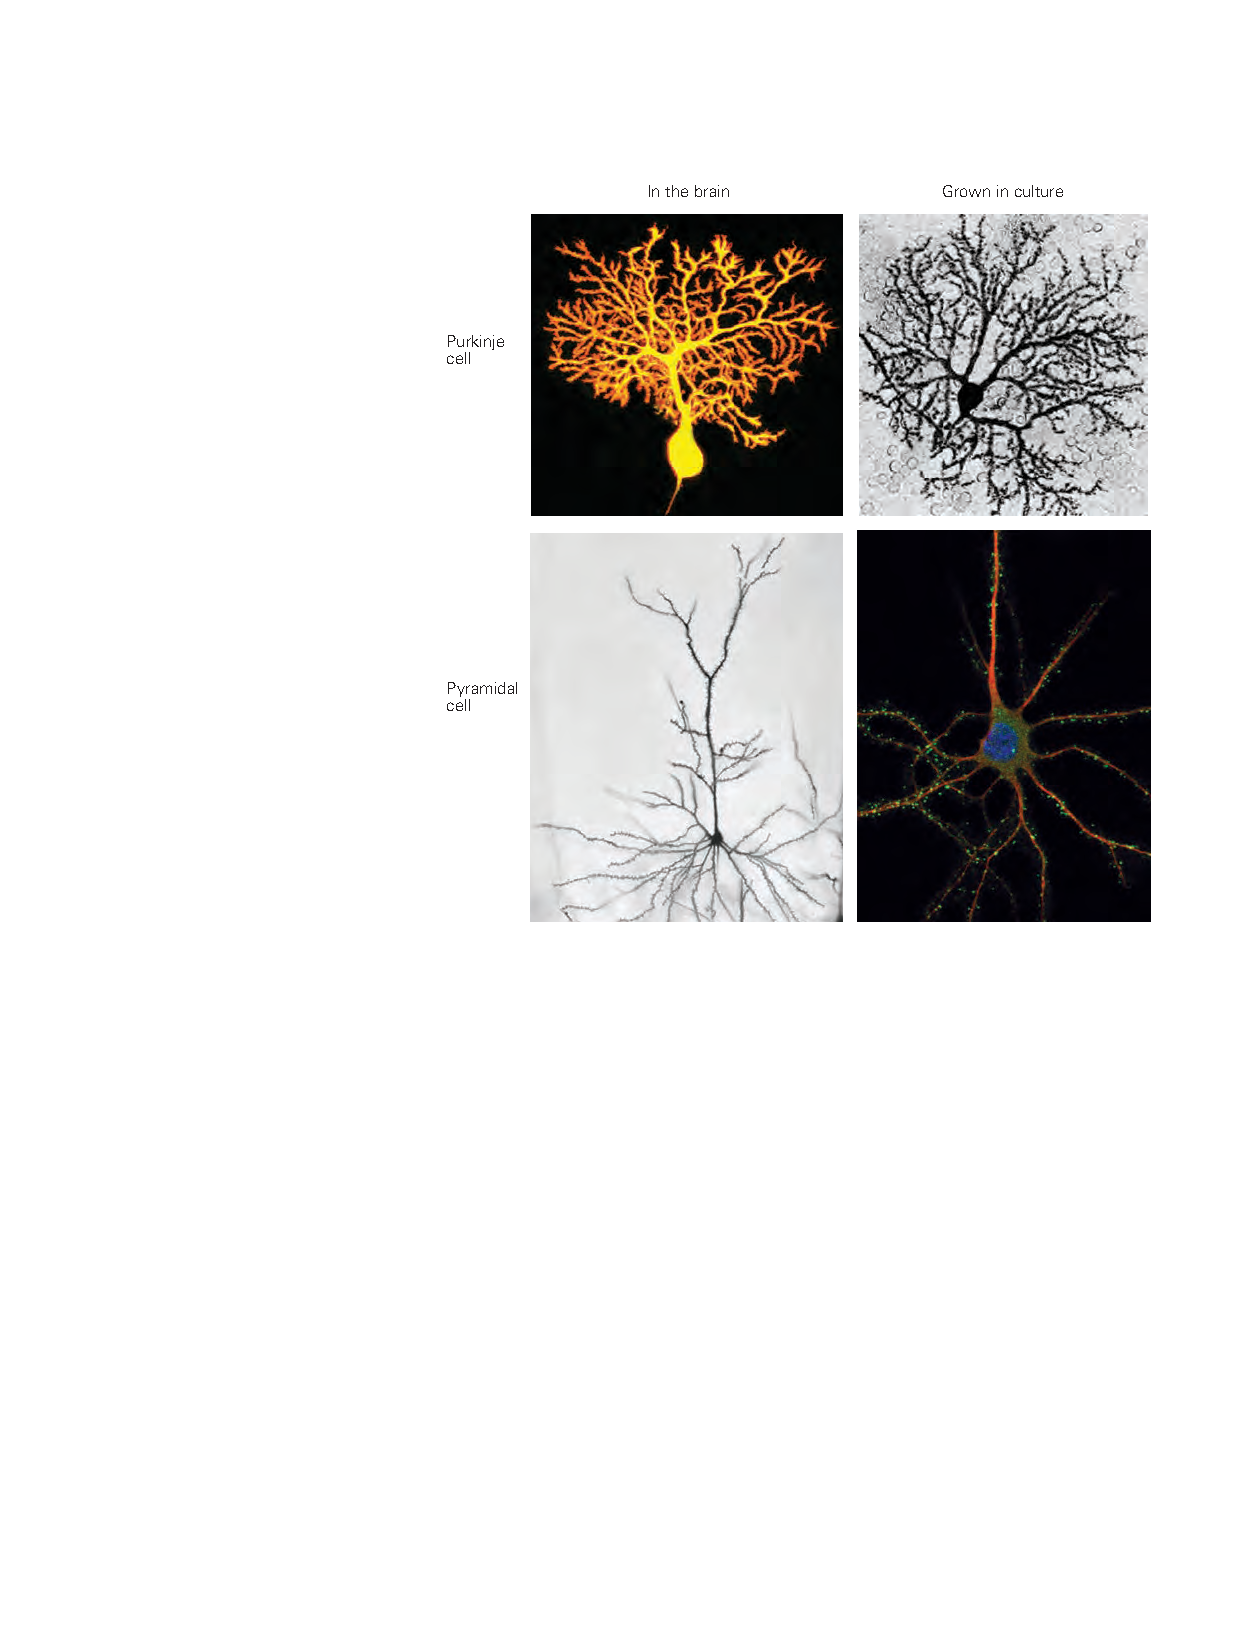
\includegraphics[width=0.7\linewidth]{chap47/fig_47_4}
	\caption{神经元的形态保存在分离的细胞培养物中。 小脑浦肯野神经元和海马锥体神经元具有独特的树突分支模式。 当这两类神经元被分离并在分离的细胞培养物中生长时,这些基本模式得到概括。 (左上图:David Becker 博士;右上角经许可转载自 Yoshio Hirabayashi;左下角经许可转载自 Terry E. Robinson;右下角经许可转载自 Kelsey Martin。)}
	\label{fig:47_4}
\end{figure}

建立树突乔木模式的第二种机制是同一细胞的其他树突识别一个树突。
在一些神经元中,树突彼此均匀分布,这种排列使它们能够有效地对输入进行采样,而不会出现大的间隙或团块(图 \ref{fig:47_5}A)。
在许多情况下,这种称为自我回避的过程是通过属于同一神经元的分支相互排斥的机制发生的。
现已发现几种细胞表面粘附分子通过以导致排斥的方式相互作用来介导自我回避(图 \ref{fig:47_5}D)。
尽管相邻膜之间的粘附相互作用会导致排斥而不是附着似乎违反直觉,但大多数细胞间相互作用的结果是由它们发起的信号决定的,而不是由粘附本身决定的,正如我们将在本章后面看到的那样。


\begin{figure}[htbp]
	\centering
	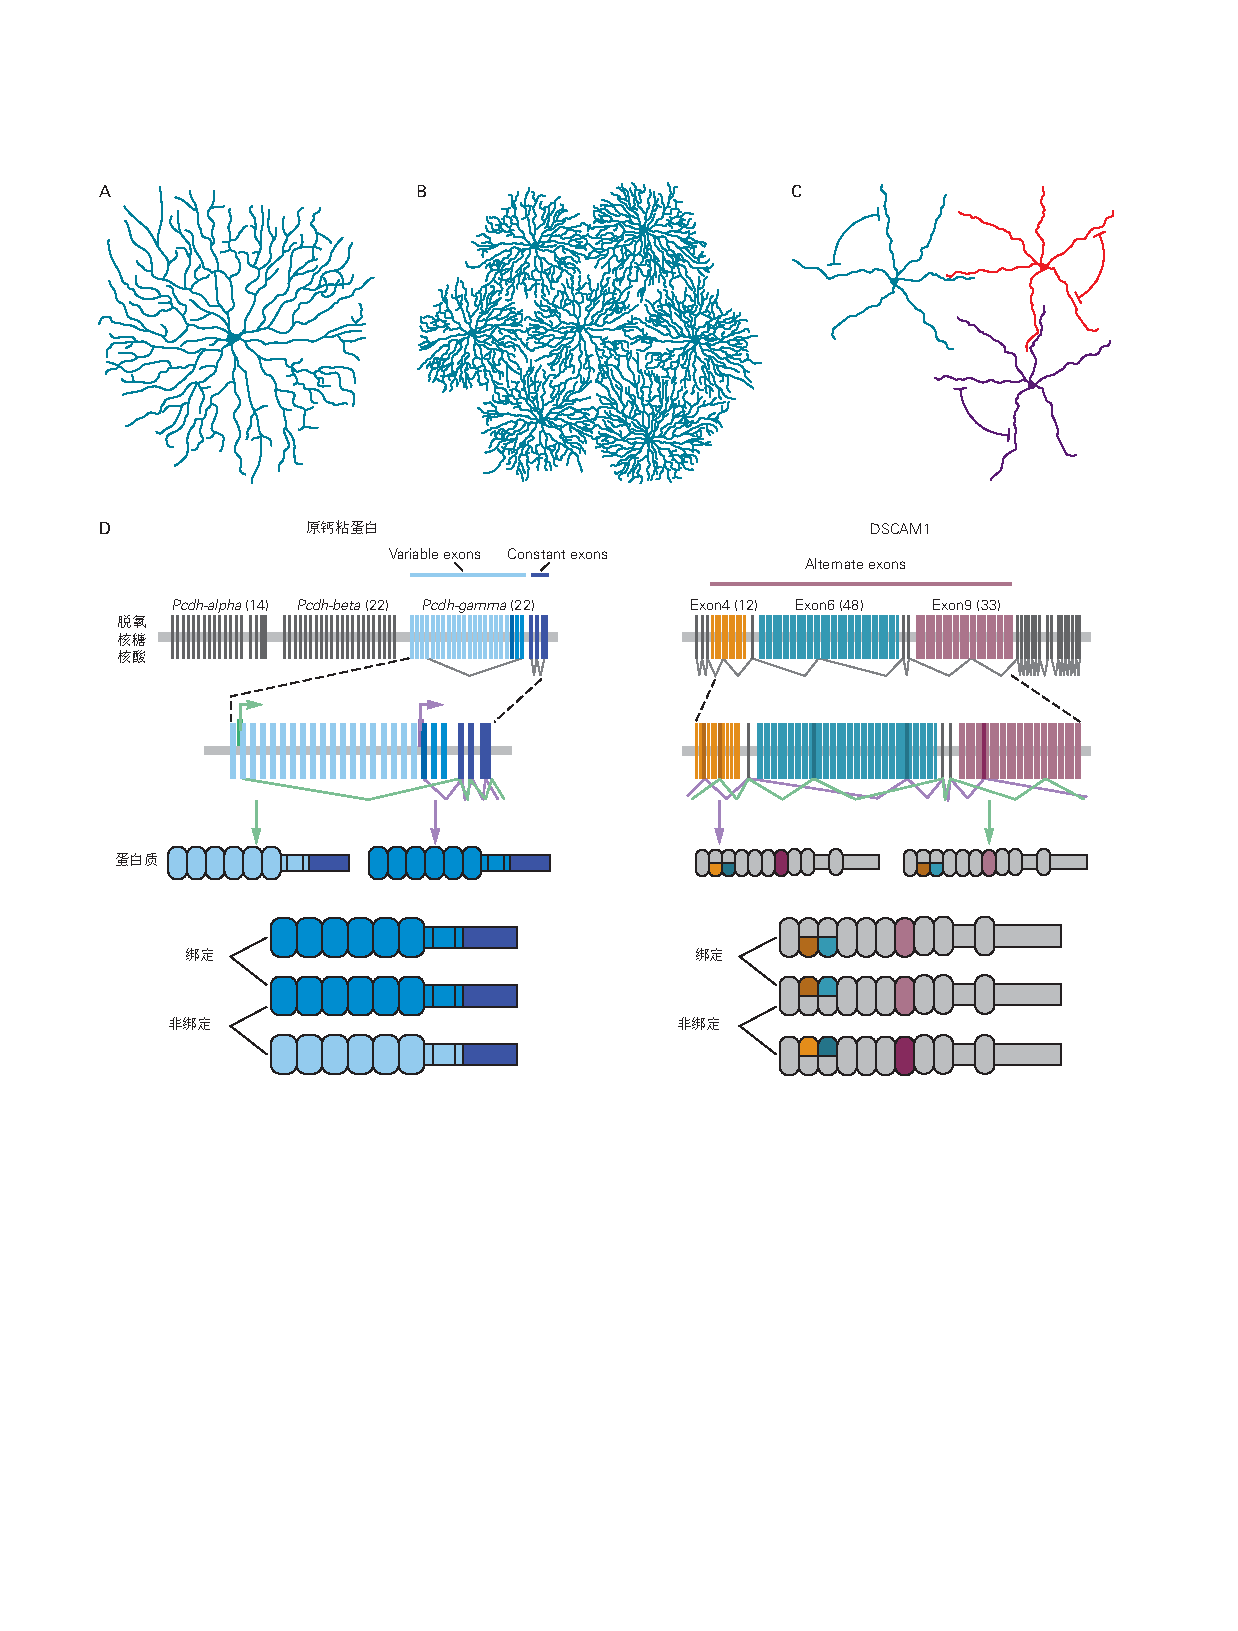
\includegraphics[width=0.95\linewidth]{chap47/fig_47_5}
	\caption{树突状分支之间的相互作用形成树突状乔木。 A. 兄弟树突之间的自我回避导致分支的间距均匀,最大限度地减少间隙和团块。 在视网膜星暴无长突细胞中,当伽马原钙粘蛋白丢失时,自我回避就会失败。 B. 树突的平铺在概念上类似于自我回避,但适用于神经元群。 它确保单一类型的相邻神经元有效地覆盖区域。 C. 自我/非自我歧视允许兄弟树突在与同一类型的其他神经元的树突自由相互作用时相互避开。 D. 通过在小鼠成簇原钙粘蛋白 (Pcdh) 位点(左)选择启动子和在果蝇 DSCAM1 位点(右)进行选择性剪接,从单个基因组复合体生成大量粘附分子。}
	\label{fig:47_5}
\end{figure}


邻近神经元的树突也提供线索。
在许多情况下,特定神经元类型的树突以最小重叠覆盖表面,这种间距模式称为平铺(图 \ref{fig:47_5}B)。
树突的平铺在概念上与自我回避有关,但在平铺中,抑制性树突相互作用发生在特定类型的神经元之间,而在自我回避中,它们发生在单个神经元的兄弟树突之间。
平铺允许每一类神经元从它支配的整个表面或区域接收信息。
通过一类神经元的树突平铺区域也避免了如果许多不同神经元的树突占据同一区域可能出现的混淆。


一个特别有趣的情况是,树突进行自我回避,但在同一类型的其他细胞的树突上形成突触。
在这种情况下,树突面临着将名义上相同的树突与名义上相同的细胞的树突区分开来的挑战性任务(图 \ref{fig:47_5}C)。
已经确定了两组介导这种自我/非自我歧视的分子:哺乳动物中的成簇原钙粘蛋白和果蝇中的 DS-CAM。
尽管它们在结构上不相关,但它们有几个共同特征(图 \ref{fig:47_5}D)。


首先,两者都由产生大量同种型的大型复杂基因编码。
果蝇 Dscam1 通过选择性剪接编码大约 38,000 种不同的蛋白质,而成簇的原钙粘蛋白编码大约 60 种蛋白质,这些蛋白质可以组装成数千种不同的多聚体。
其次,几乎所有的亚型都同嗜结合;
例如,一个树突表面上的原钙粘蛋白 γa1 与相邻膜上的原钙粘蛋白 γa1 结合良好,但与其他同种型的结合很差。
第三,以仍未完全理解的方式,群体中的每个神经元表达所有可能的 Dscam1 或原钙粘蛋白亚型的随机子集。
考虑到大量的异构体,单个神经元不太可能在其细胞表面表达相同的异构体集。
结果是群体中每个神经元的树突同胞树突结合,导致排斥和自我回避,而它们与邻近神经元的树突结合不良,使其他识别系统能够促进突触发生。


总之,我们所描述的机制以及许多其他机制通过内在机制和细胞外机制的结合建立了整体树枝化模式。
对于树突,外在模式信号决定了神经元的形态。
对于我们接下来要考虑的轴突,信号引导轴突到达它们的目标。



\section{生长锥是一种感觉传感器和运动结构}

一旦轴突形成,它就开始向其突触目标生长。
负责轴突生长的关键神经元元素是轴突尖端的一种特殊结构,称为生长锥。
轴突和树突都使用生长锥来伸长,但与轴突相关的生长锥已得到更深入的研究。


拉蒙·卡哈尔 (Ramón y Cajal) 发现了生长锥,并对它负责轴突寻路有了关键的认识。
仅以静态图像作为灵感(图 \ref{fig:47_6}A),他设想生长锥“具有精湛的化学敏感性、快速的变形虫运动和一定的动力,因此它能够继续前进并克服遇到的障碍 它的方式。 . . 直到到达目的地。”


\begin{figure}[htbp]
	\centering
	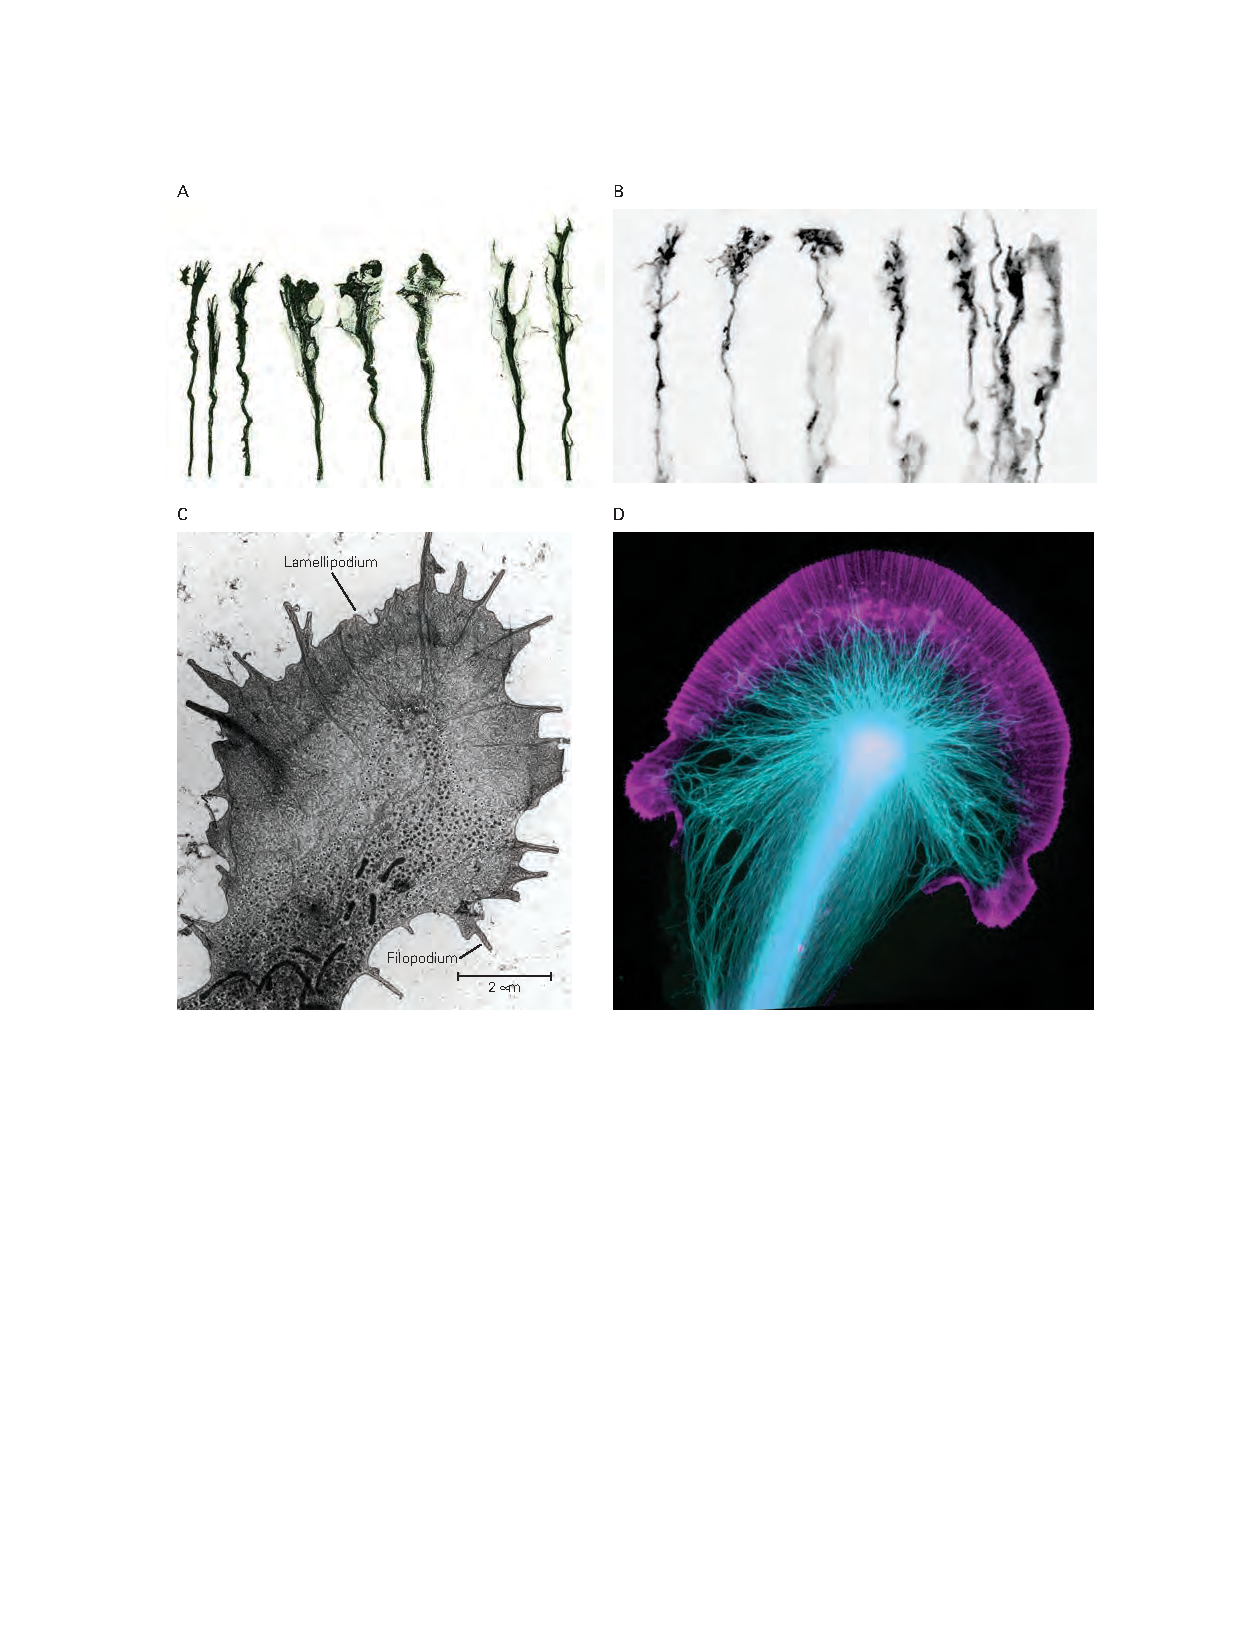
\includegraphics[width=0.8\linewidth]{chap47/fig_47_6}
	\caption{神经元生长锥。 A. Santiago Ramón y Cajal 绘制的生长锥图,他发现了这些细胞结构并推断了它们的功能。 B. 在小鼠中染料标记的视网膜神经节神经元中可视化的生长锥。 请注意与卡哈尔绘画的相似之处。 (经许可转载自 Carol Mason 和 Pierre Godement。)C. 生长锥的三个主要区域——丝状伪足、片状伪足和中央核心——通过整体扫描电子显微镜显示。 (经许可转载自 Bridgman 和 Dailey 1989。许可通过 Copyright Clearance Center, Inc. 转达) D. 来自海兔的神经元的生长锥,其中肌动蛋白和微管蛋白已经显现。 肌动蛋白(紫色)集中在片状伪足和丝状伪足中,而微管蛋白和微管(海蓝宝石)集中在中央核心。 (经许可转载自 Paul Forscher 和 Dylan Burnette。)}
	\label{fig:47_6}
\end{figure}


过去一个世纪的许多研究证实了 Ramón y Cajal 的直觉。
我们现在知道,生长锥既是一种从环境中接收定向线索的感觉结构,也是一种活动驱动轴突伸长的运动结构。
Ramón y Cajal 还思考了“在这些过程出现之前有哪些神秘力量…… . . 促进它们的生长和分枝。 . . 并最终建立起那些原生质之吻。 . . 这似乎构成了一个史诗般的爱情故事的最后狂喜。” 
用更现代和平淡无奇的术语来说,我们现在知道生长锥通过将正负信号转变成调节细胞骨架的信号来引导轴突,从而确定轴突向其目标生长的过程和速度,它将在此处形成突触。


生长锥具有三个主要隔间。
它们的中央核心富含微管、线粒体和其他细胞器。
从生长锥体伸出称为丝状伪足的细长延伸物。
丝状伪足之间是片状伪足,它们也能运动,并赋予生长锥特有的褶皱外观(图 47–6C、D)。


生长锥体通过它们的丝状伪足感知环境信号:杆状、富含肌动蛋白、高度运动的膜限制结构。
它们的表面膜带有分子受体,这些分子充当轴突的定向信号。
它们的长度——在某些情况下为数十微米——允许丝状伪足在生长核心的中央核心之前对环境进行采样。
它们的快速移动使它们能够编制一份详细的环境清单,它们的灵活性使它们能够在细胞和其他障碍物周围导航。


当丝状伪足遇到环境中的信号时,生长锥会受到刺激前进、后退或转动。
几个马达为这些定向行为提供动力。
一种力量来源是肌动蛋白沿肌球蛋白的运动,这种相互作用类似于为骨骼肌纤维收缩提供动力的相互作用,尽管神经元的肌动蛋白和肌球蛋白与肌肉中的不同。
肌动蛋白单体组装成聚合物丝也有助于丝足延伸的推进力。
由于肌动蛋白丝在丝状伪足的基部不断解聚,聚合和解聚的平衡使丝状伪足向前移动而不会变长。
解聚在生长锥前进期间减慢,导致更大的净向前运动。
膜沿基底的运动提供了另一种向前运动的来源。


每种类型的分子马达对生长锥推进的贡献可能因情况而异。
然而,最后一步涉及微管从生长锥的中央核心流入新延伸的尖端,从而使生长锥向前移动并在其后留下新的轴突片段。
新的片状伪足和丝状伪足在前进的生长锥中形成并且循环重复(图 \ref{fig:47_7})。


\begin{figure}[htbp]
	\centering
	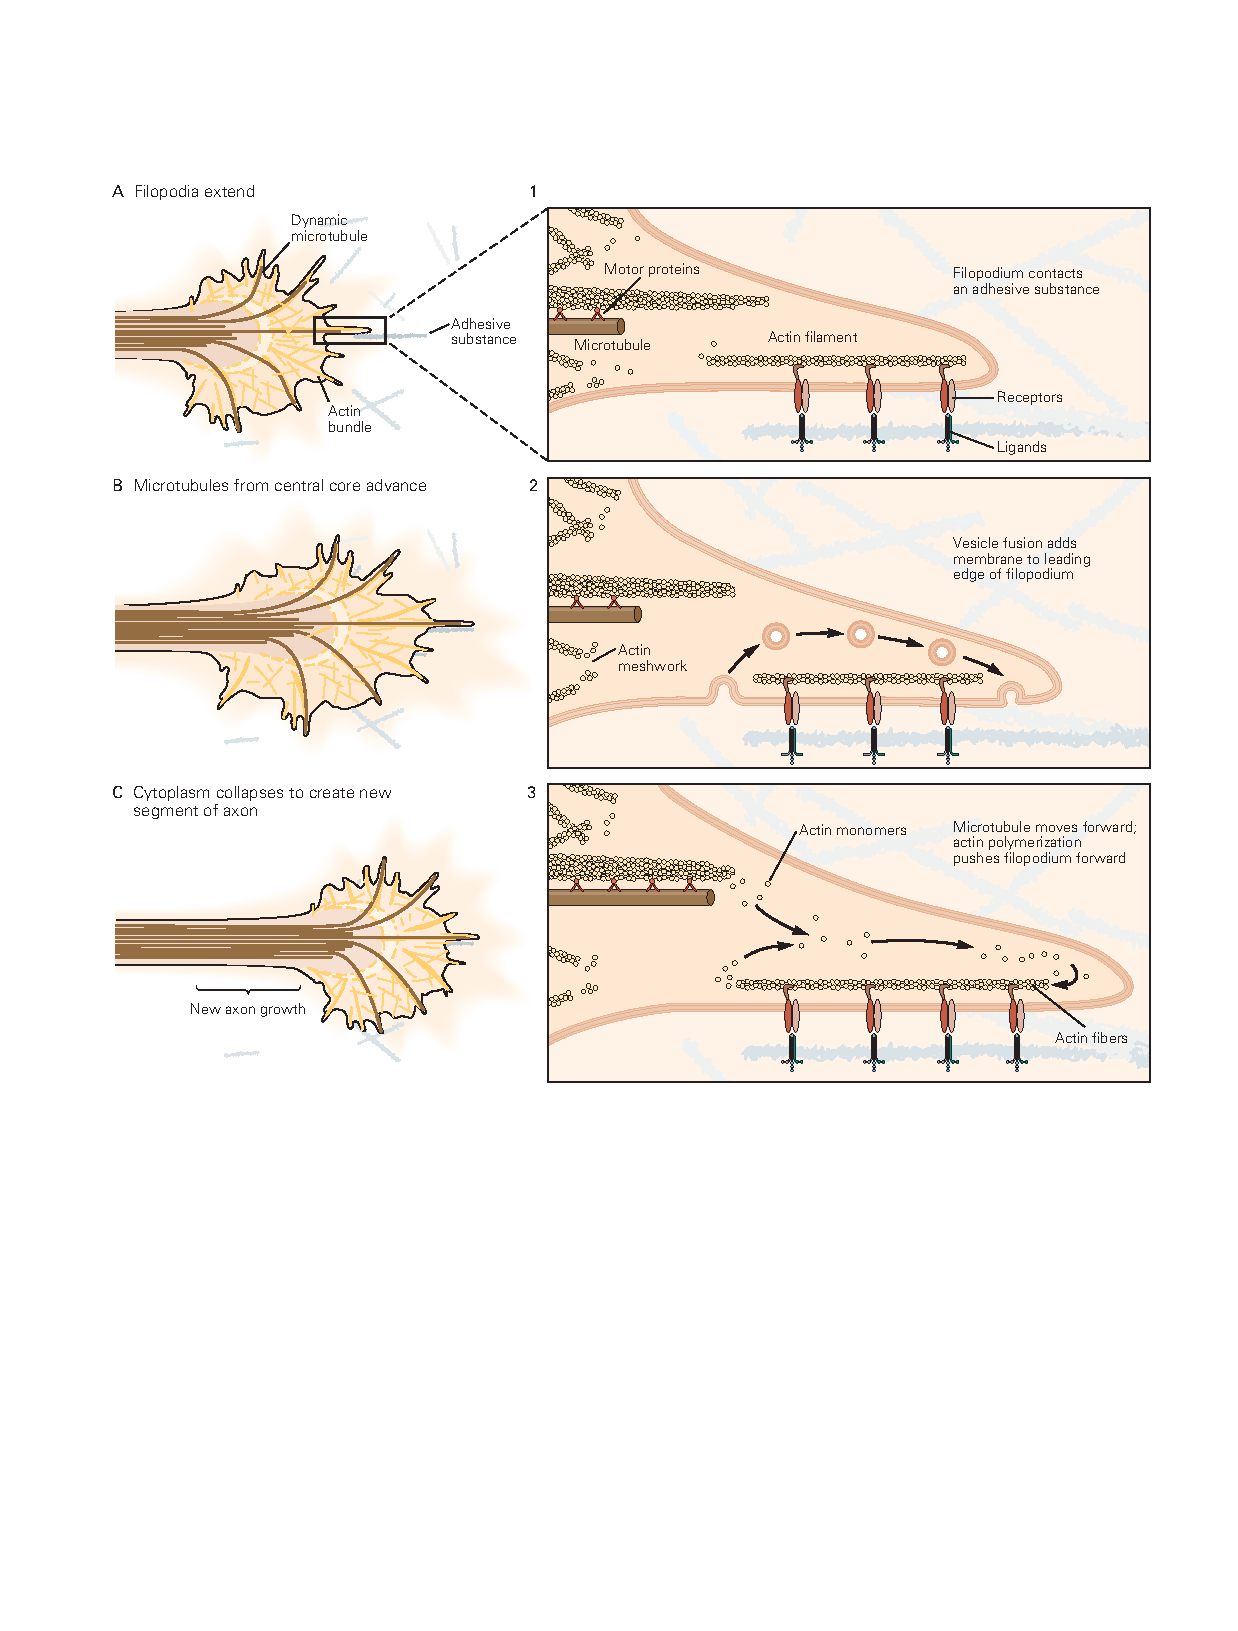
\includegraphics[width=0.9\linewidth]{chap47/fig_47_7}
	\caption{生长锥在细胞马达的控制下前进。 (经许可改编自 Heidemann 1996。版权所有 © 1996 Academic Press Inc.) A. 丝状伪足接触粘性提示并收缩,从而向前拉动生长锥 (1)。 肌动蛋白丝在丝状足的前缘聚集,在后缘分解,沿途与肌球蛋白相互作用 (2)。 肌动蛋白聚合推动丝足向前 (3)。 肌动蛋白逆行产生的力推动丝状伪足向前。 胞吐作用将膜添加到丝状足的前缘,并提供新的粘附受体以保持牵引力。 在丝状足的背面回收膜。 肌动蛋白聚合物与质膜上的粘附分子相连。 B. 这些马达的联合作用产生了一个空隙,由来自中央核心的微管推进填充。 C. 单个微管凝结成粗束,细胞质围绕它们塌陷,形成新的轴突轴段。}
	\label{fig:47_7}
\end{figure}


只有当生长锥的运动动作与其感觉功能相关联时,才能进行准确的寻路。
因此,至关重要的是,丝状伪足上的识别蛋白是信号诱导受体,而不仅仅是介导粘附的结合部分。
配体与其受体的结合以多种方式影响生长。
在某些情况下,它通过受体的细胞内结构域直接与细胞骨架结合(图 \ref{fig:47_7})。
当整合素受体结合与相邻细胞表面或细胞外基质相关的分子时,它们会与生长锥中的肌动蛋白偶联,从而影响运动性。


同样重要甚至更重要的是配体结合刺激作为第二信使发挥作用的可溶性细胞内分子的形成、积累甚至分解的能力。
这些第二信使影响细胞骨架的组织,并以此方式调节生长锥运动的方向和速度。


一个重要的第二信使是钙。
生长锥中的钙浓度受丝状伪足上受体激活的调节,这会影响细胞骨架的组织,进而调节运动性。
生长锥运动在狭窄的钙浓度范围内是最佳的,称为设定点。
生长锥一侧丝状伪足的激活导致整个生长锥的钙浓度梯度,为生长方向的变化提供了可能的基础。


连接受体和运动分子的其他第二信使包括环核苷酸,它调节酶的活性,例如蛋白激酶、蛋白磷酸酶和 rho 家族鸟苷三磷酸酶 (GTP 酶)。
反过来,这些信使和酶调节调节肌动蛋白丝聚合和解聚的蛋白质的活性,从而促进或抑制轴突延伸。


细胞内信号在生长锥运动和方向中的关键作用可以使用在培养物中生长的胚胎神经元来证明。
将生长因子应用于生长锥的一侧会激活局部受体,并导致生长锥向信号源延伸和转向。
本质上,该因子吸引了生长锥。
然而,当神经元中的环磷酸腺苷 (cAMP) 水平降低时,相同的刺激会起到驱虫剂的作用,并且生长锥会远离信号(图 \ref{fig:47_8}A)。
当第二信使环鸟苷 3',5'-单磷酸 (cGMP) 的水平升高时,其他排斥因素可能变得有吸引力。


\begin{figure}[htbp]
	\centering
	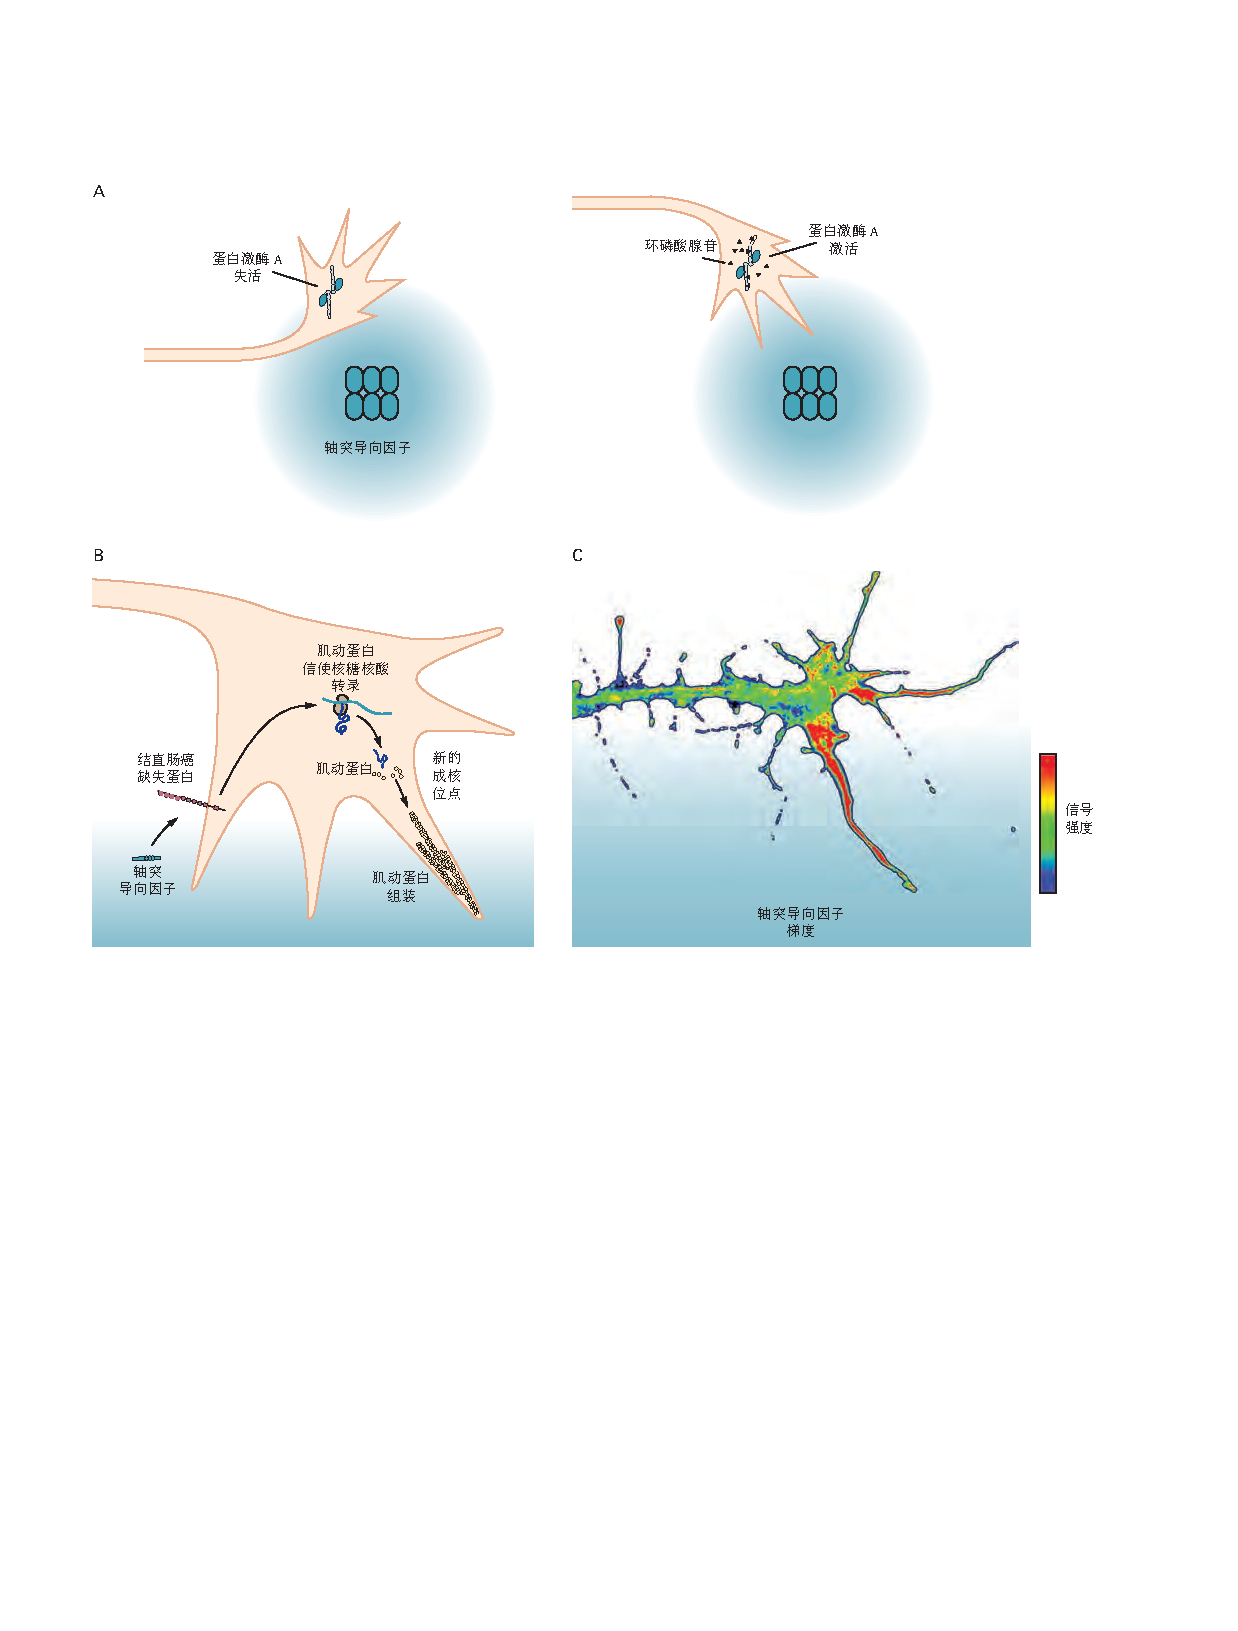
\includegraphics[width=0.9\linewidth]{chap47/fig_47_8}
	\caption{细胞内调节蛋白水平的变化可以决定相同的外在信号是吸引还是排斥生长锥。 A. 蛋白激酶 A (PKA) 活性的状态可以改变生长锥对细胞外定向因子的反应,在本例中为蛋白质 netrin。 当 PKA 活性和细胞内环磷酸腺苷 (cAMP) 水平较低时,生长锥会被 netrin 排斥。 当 PKA 活性高时,细胞内 cAMP 的升高导致生长锥被吸引到局部 netrin 来源。 (经许可改编自 Ming 等人,1997 年。)B. 生长锥受体的 Netrin 激活(在结肠癌 DCC 中缺失)导致肌动蛋白的局部合成,从而导致转向。 C. 生长锥的免疫组织化学分析显示局部合成肌动蛋白以响应局部应用 netrin。 (经许可转载自 Christine Holt。经许可改编自 Leung 等人,2006 年。)}
	\label{fig:47_8}
\end{figure}


最近,另一种将引导分子耦合到生长锥行为的机制已经曝光。
长期以来,人们认为所有神经元蛋白质的合成都发生在细胞体中,但我们现在知道,生长锥(以及一些树突)含有蛋白质合成机制,包括信使 RNA 的一个子集。
这些分子发挥重要作用的初步证据来自轴突与母细胞体分离的实验。
生长锥继续前进了几个小时; 它们可以被刺激转向或远离当地的引导分子库,而这些行为被蛋白质合成抑制剂所废除。
局部蛋白质合成受第二信使的调节,第二信使响应生长锥上引导受体的激活而产生(图 \ref{fig:47_8})。
这种机制导致在需要的时间和地点精确地合成新的运动蛋白。
因此,生长锥有许多策略和机制来整合分子信号以在特定方向引导轴突。



\section{分子线索引导轴突到达目标}

在 20 世纪的大部分时间里,关于生长锥如何通过胚胎地形到达目标的两种截然不同的观点的倡导者之间展开了激烈的辩论。
20 世纪之交,生理学家 J. N. Langley 首次阐述了轴突导向的分子观点。
但到了 1930 年代,包括保罗·韦斯在内的许多著名生物学家认为,轴突的生长本质上是随机的,适当的连接之所以能够持续存在,主要是因为轴突及其目标细胞中的电活动具有生产力,匹配模式。


在我们的分子时代,魏斯的想法看似简单,但在当时并非没有道理。
在组织培养中,轴突优先沿着机械不连续点(盖玻片上的划痕和凸起)生长,胚胎神经干通常与固体支撑物(血管或软骨)对齐。
Weiss 认为机械引导(称为立体定向)可以解释轴突模式,这似乎是合乎逻辑的。
今天,我们对电信号可用于改变电流在计算机中流动的方式而无需重新焊接连接的想法感到非常满意。
同样,活动模式和经验可以加强或削弱神经连接,而不需要形成新的轴突通路。
那么,为什么不考虑建立适当联系所涉及的一致活动(被 Weiss 称为共振)呢?


今天,很少有科学家认为立体定向或共振是神经回路初始模式形成的关键力量。
使观点转向支持分子观点的转折点是 1940 年代 Roger Sperry(具有讽刺意味的是,他是 Weiss 的学生)用青蛙和其他两栖动物进行的实验。
斯佩里操纵由视网膜神经节细胞的轴突从眼睛传送到大脑的信息。
这些轴突终止于它们的目标区域——丘脑中的外侧膝状体和中脑中的上丘(在低等脊椎动物中称为视顶盖)——以这样一种方式创建了有序的视野视网膜专题图。


由于眼睛的光学系统,视网膜上的视觉图像是视野的倒置。
视网膜神经节细胞通过其轴突终止于视顶盖的模式重新反转图像,视顶盖是青蛙大脑中的主要视觉中心(图 \ref{fig:47_9}A)。
如果视神经被切断,动物就会失明。
在低等脊椎动物中,切断的视网膜轴突可以重新建立对顶盖的投射,从而恢复视力。
哺乳动物的情况并非如此,我们将在第 \ref{chap:chap50} 章中讨论。


\begin{figure}[htbp]
	\centering
	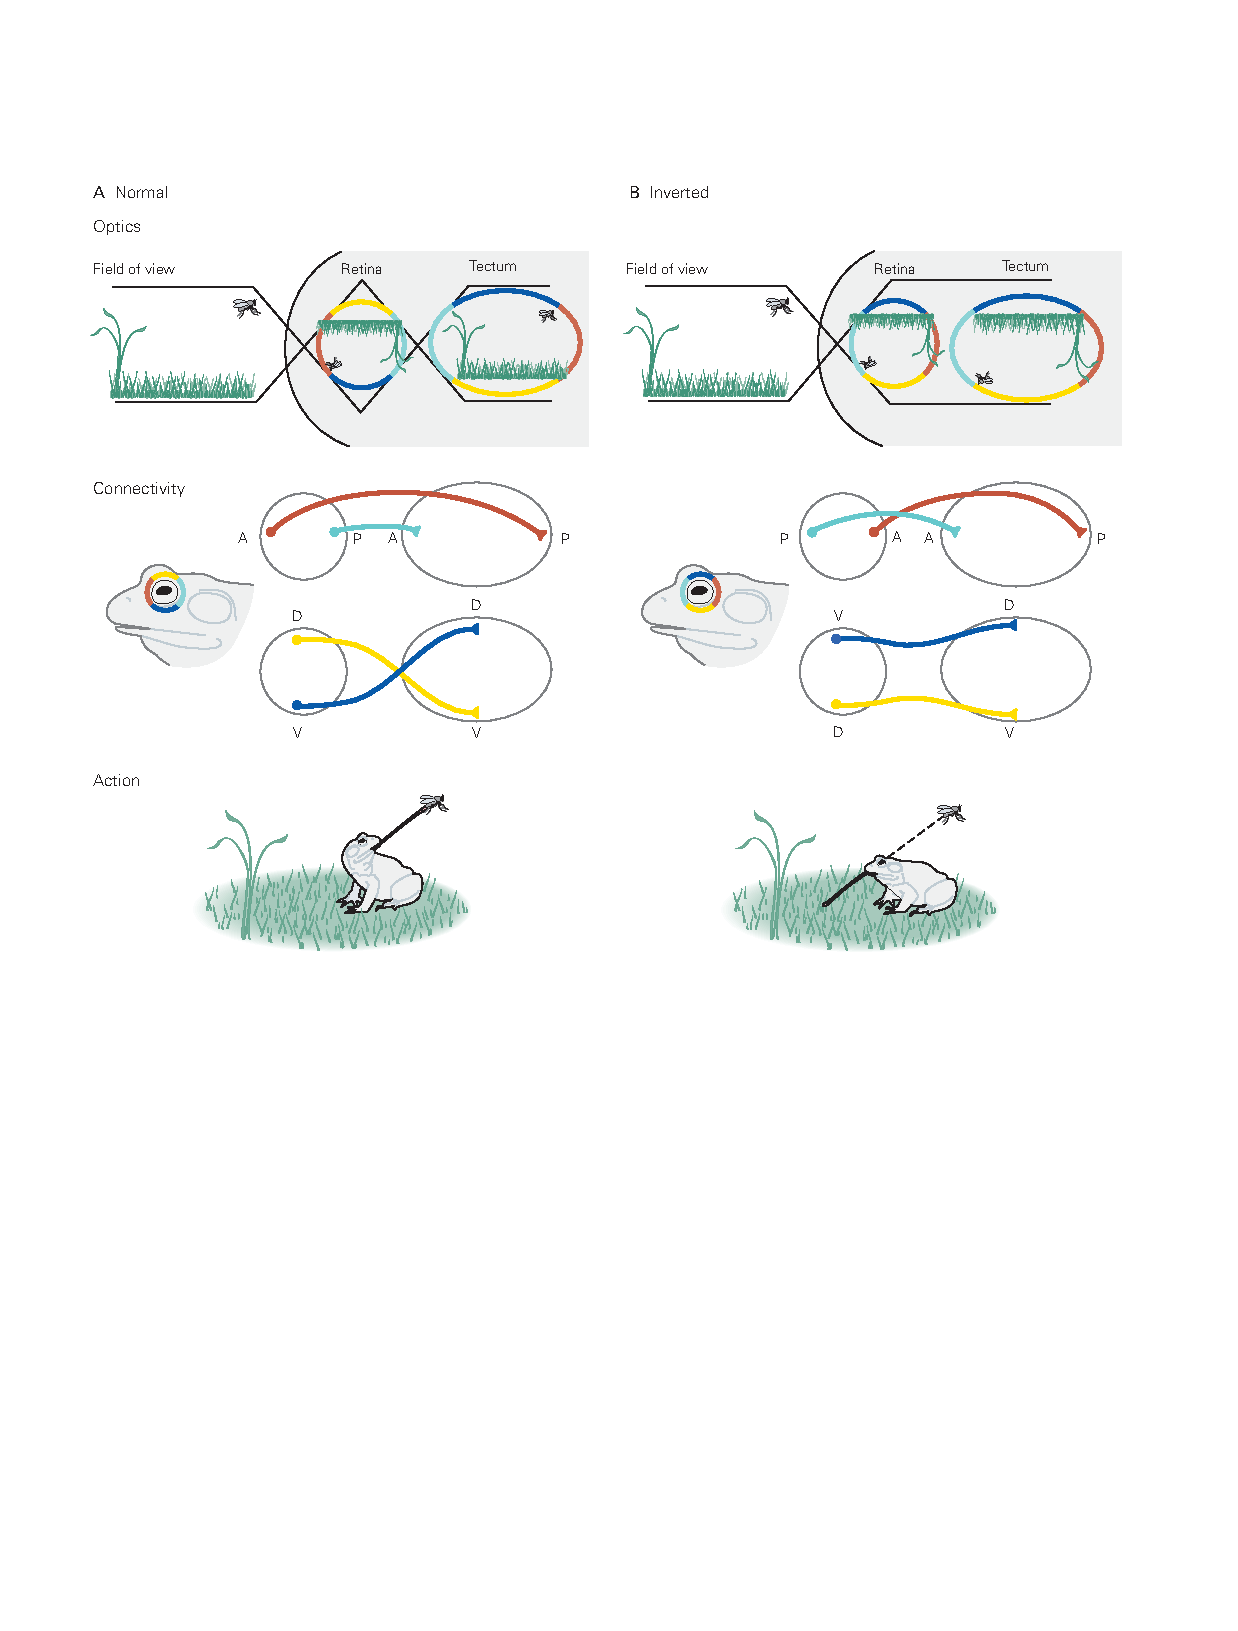
\includegraphics[width=0.9\linewidth]{chap47/fig_47_9}
	\caption{罗杰·斯佩里 (Roger Sperry) 关于视觉系统再生的经典实验为连接线路中的化学亲和力提供了证据。 A. 在青蛙的视觉系统中,晶状体将倒置的视觉图像投射到视网膜上,然后视神经将图像通过额外的倒置传递到视顶盖。 视网膜输入到顶盖的空间排列允许这种转移。 前视网膜中的神经元将轴突投射到后顶盖,而后视网膜中的神经元投射到前顶盖。 同样,背侧视网膜中的神经元投射到腹侧顶盖,而腹侧视网膜中的神经元投射到背侧顶盖。 因此,视觉引导的行为(这里是抓苍蝇)是准确的。 (缩写:A,前部;D,背侧;P,后部;V,腹侧。)B. 如果视神经被切断,并且在神经再生之前通过手术将眼睛在其插座中旋转,则视觉引导行为是异常的。 当一只苍蝇出现在头顶时,青蛙会在下方感知它,反之亦然。 行为反射的倒置是由再生的视网膜轴突与其原始目标的连接引起的,尽管这些连接现在将一个倒置的、不合适的世界地图传输到大脑中。}
	\label{fig:47_9}
\end{figure}


Sperry 的关键实验是切断青蛙的视神经,然后在神经再生之前将眼球在眼窝中旋转 180°。
值得注意的是,这只青蛙对视觉输入表现出了有序的反应,但这种行为是错误的。
当青蛙在地上看到一只苍蝇时,它会跳起来,当在它头顶上方有一只苍蝇时,它会向下击打(图 \ref{fig:47_9}B)。
重要的是,这种动物从未学会改正错误。
斯佩里提出——后来用解剖学和生理学方法证实——视网膜轴突重新支配了它们原来的顶盖目标,尽管这些连接为大脑提供了导致异常行为的错误空间信息。
这些实验的推论是,轴突及其目标之间的识别依赖于分子匹配,而不是随机连接的功能验证和改进。


但魏斯的想法绝不会过时。
事实上,我们现在认识到神经回路的活动可以在塑造连通性方面发挥关键作用。
目前的观点是,分子匹配在胚胎发育过程中占主导地位,而活动和经验会在回路形成后对其进行修改。
在本章和下一章中,我们描述了指导神经连接形成的分子线索,然后在第 \ref{chap:chap49} 章中,我们研究了活动和经验在微调突触连接中的作用。


Sperry 的猜想,通常称为化学特异性假说,促使发育神经生物学家寻找轴突和突触“识别分子”。
在最初的几十年里,成功是有限的,部分原因是这些分子数量很少,并且存在于神经元的离散子集中,并且没有从复杂组织中分离稀有分子的有效方法。
最终,生化和分子生物学方法的进步使这项任务变得更加可行,并且现在已经发现了许多参与将轴突引导至其目标的蛋白质。
这些蛋白质通常由成对的配体和受体组成:配体由细胞沿着轴突所遵循的路径呈现,受体由生长锥本身呈现。


用最一般的术语来说,指导线索可以出现在细胞表面、细胞外基质或可溶性形式中。
如上所述(图 \ref{fig:47_8}),它们与嵌入生长锥膜中的受体相互作用,以促进或抑制轴突的生长。
大多数受体都有一个胞外结构域,可以选择性地结合同源配体,以及一个胞内结构域,可以直接或通过第二信使等中间体与细胞骨架偶联。
配体可以加速或减缓生长。
出现在生长锥一侧的配体可导致局部激活或抑制,从而导致转向。
这样,环境线索的局部分布决定了前进生长锥的路径。


由于这些最近的发现,轴突引导——一个多年前出现的神秘过程——现在可以被视为蛋白质-蛋白质相互作用的有序结果,它指示生长锥生长、转动、分支或停止(图 47- 10, 11)。
当以空间精度呈现时,这套有限的指令足以以精致微妙的方式编排生长锥行为。
因此,可以通过描述配体的呈现方式和位置以及生长锥如何整合此信息以产生有序反应来解释轴突引导。
在本章的其余部分,我们通过描述两种类型的轴突的行程来说明所学到的经验教训:
视网膜神经节神经元的轴突和脊髓中特定类别的感觉中继神经元的轴突。



\section{视网膜神经节轴突的生长以一系列离散步骤为导向}

斯佩里的实验暗示了轴突引导线索的存在,但没有揭示它们的位置或工作方式。
有一段时间,一个突出的观点是识别主要发生在目标处或附近,机械力或远程趋化因子足以使轴突到达目标附近。


我们现在知道,轴突通过一系列不连续的步骤到达远处的目标,沿着它们的路线以紧密的间隔做出频繁的决定。
为了说明这一点,我们将更详细地追溯斯佩里试图理解的路径,即视网膜轴突生长到视顶盖的路径。



\subsection{生长锥在视交叉处发散}

视网膜神经节细胞轴突的首要任务是离开视网膜。
当它进入光纤层时,它沿着视网膜边缘的基底层和神经胶质端足延伸。
轴突的生长从一开始就是定向的,表明它可以读取环境中的定向线索。
当它接近视网膜中心时,它受到从视神经乳头(视神经与视网膜本身的交界处)发出的引诱剂的影响,引导它进入视柄。 然后它沿着视神经走向大脑(图 \ref{fig:47_12})。


\begin{figure}[htbp]
	\centering
	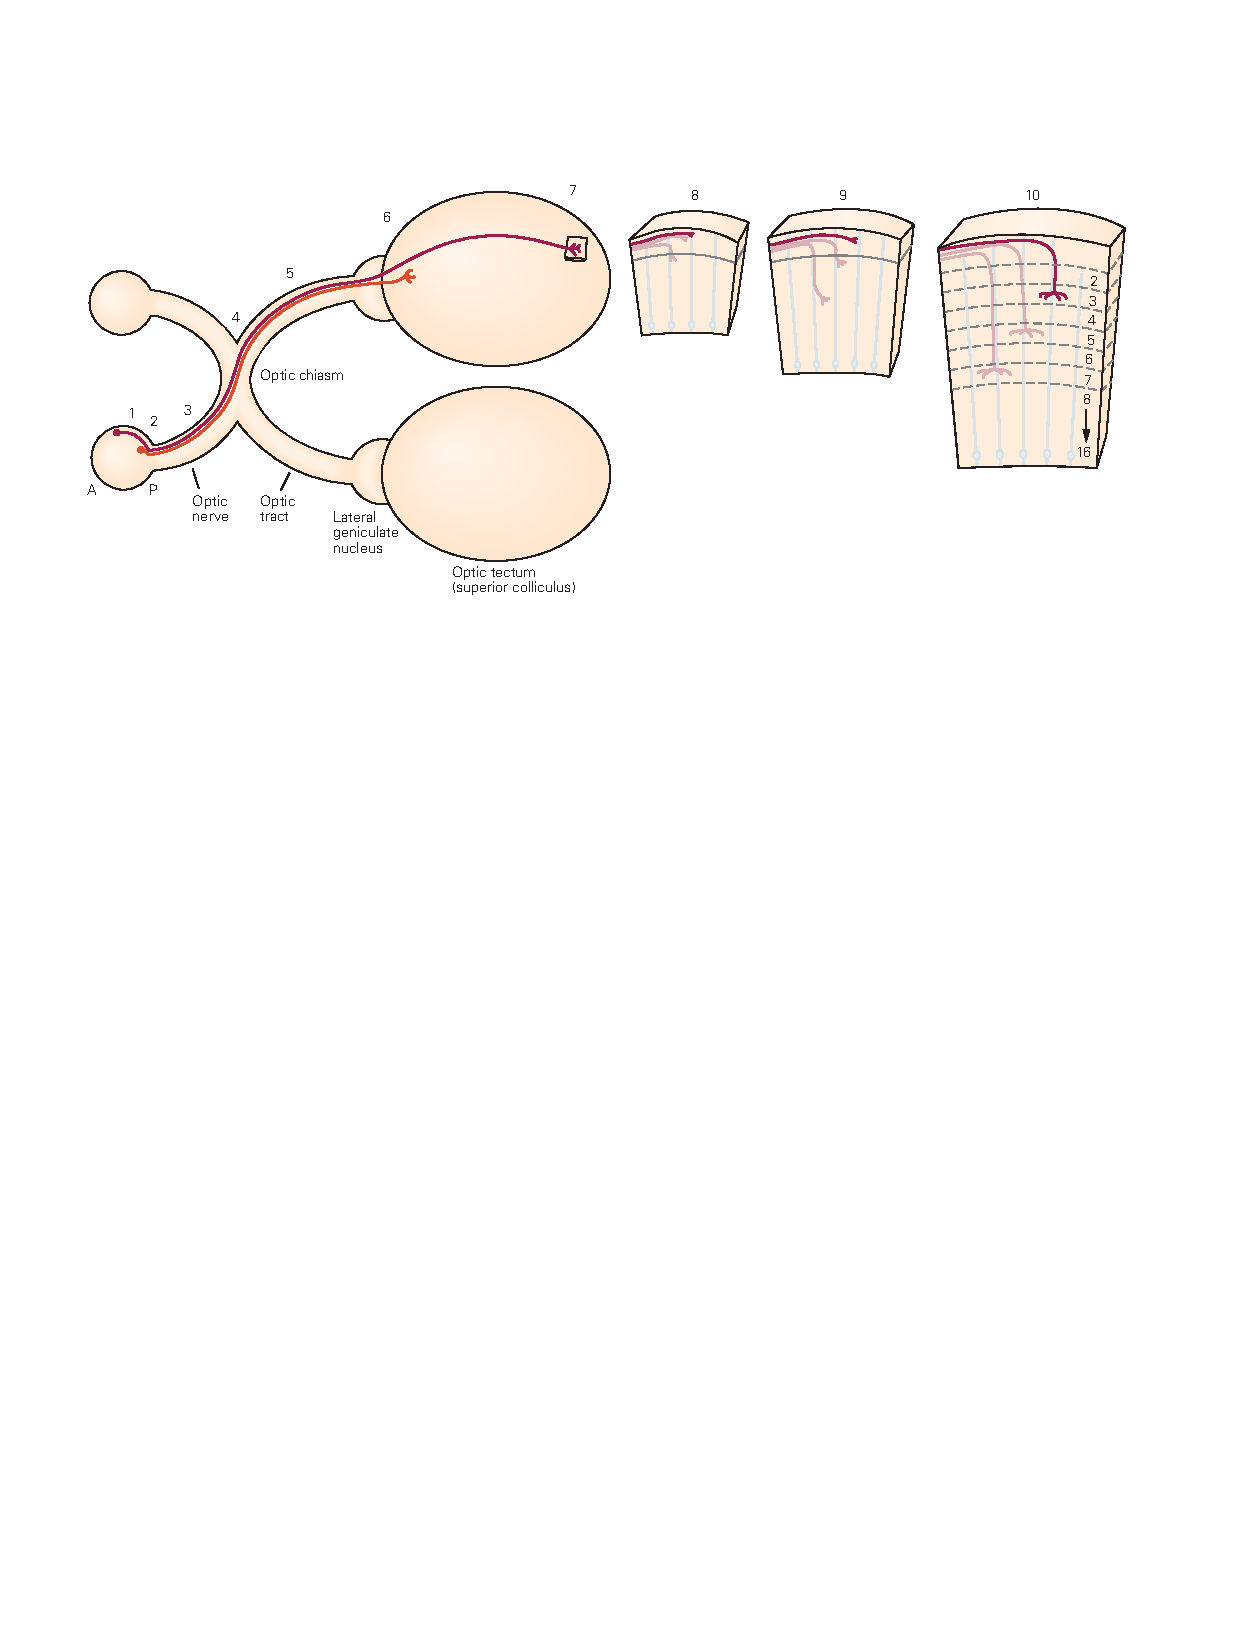
\includegraphics[width=0.95\linewidth]{chap47/fig_47_12}
	\caption{视网膜神经节细胞的轴突以不连续的步骤生长到视顶盖。 图中显示了两个神经元,它们携带来自视网膜鼻部的信息。 一个的轴突穿过视交叉到达对侧视顶盖。 另一个的轴突也穿过视交叉但投射到外侧膝状体核。 这些数字表示轴突旅程中的重要地标。 生长的轴突指向视神经乳头(神经与视网膜的交界处)(1),进入视神经 (2),延伸穿过视神经 (3),转向保持同侧(未显示) 或在视交叉 (4) 处穿过对侧,延伸穿过视束 (5),进入视顶盖或外侧膝状体核(未显示)(6),导航至适当的头尾侧和背腹侧位置 顶盖 (7),转向进入神经网(如图所示,在小鸡中下降;在哺乳动物中上升)(8),在形成基本末端乔木的适当层停止 (9),最后进行改造 (10)。 (缩写:A,前部;P,后部)。}
	\label{fig:47_12}
\end{figure}


沿着这条路线行进的第一个轴突跟随视柄细胞,视柄细胞是连接视网膜和它起源的间脑的神经管的雏形。
然后,这些“先驱”轴突充当后来到达的轴突的支架,这些轴突只需跟随它们的前辈就能够准确地延伸(参见图 \ref{fig:47_10} 中的“束缚”)。
然而,一旦它们到达视交叉,视网膜轴突就必须做出选择。
由每只眼睛的鼻侧视网膜中的神经元产生的轴突穿过视交叉并前进到大脑的另一侧,而来自颞半部的轴突在到达视交叉时发生偏转,因此停留在大脑的同一侧(图 \ref{fig:47_13} A)。


\begin{figure}[htbp]
	\centering
	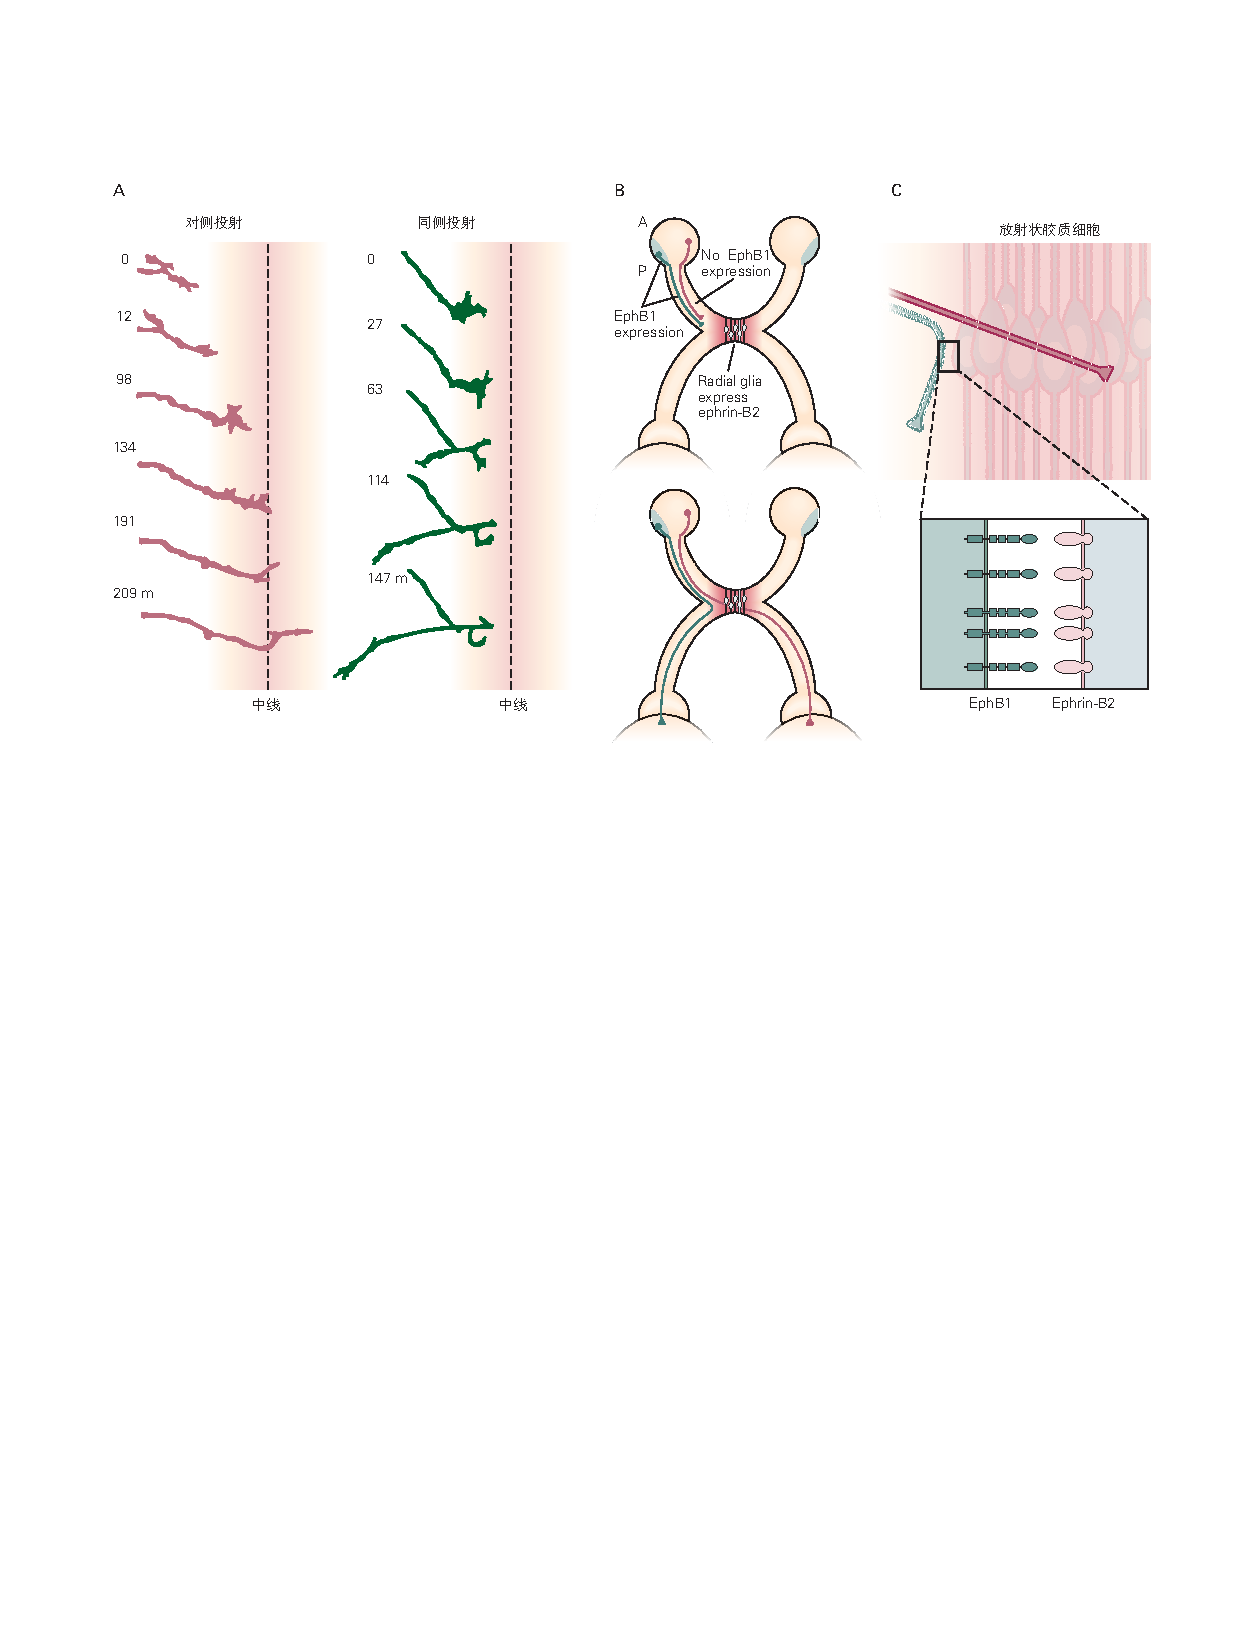
\includegraphics[width=0.95\linewidth]{chap47/fig_47_13}
	\caption{视网膜神经节神经元的轴突在到达视交叉时发散。 A. 延时系列显示轴突接近中线。 源自鼻侧视网膜的轴突穿过视交叉并投射到对侧顶盖(左)。 相比之下,来自颞侧视网膜的轴突到达视交叉但未能交叉,因此投射到同侧顶盖(右)。 (经许可转载自 Godement、Wang 和 Mason 1994。)B. 表达酪氨酸激酶受体 EphB1 的颞侧视网膜神经元轴突在视交叉处遇到由中线放射状神经胶质细胞表达的 ephrin-B2 和 所以不能越过中线。 缺乏 EphB1 受体的鼻侧视网膜神经元的轴突不受 ephrin-B2 存在的影响,并交叉到对侧。 (缩写:A,前部;P,后部。)C. 说明视交叉处视网膜神经节细胞轴突轨迹的高倍视图。}
	\label{fig:47_13}
\end{figure}


\begin{figure}[htbp]
	\centering
	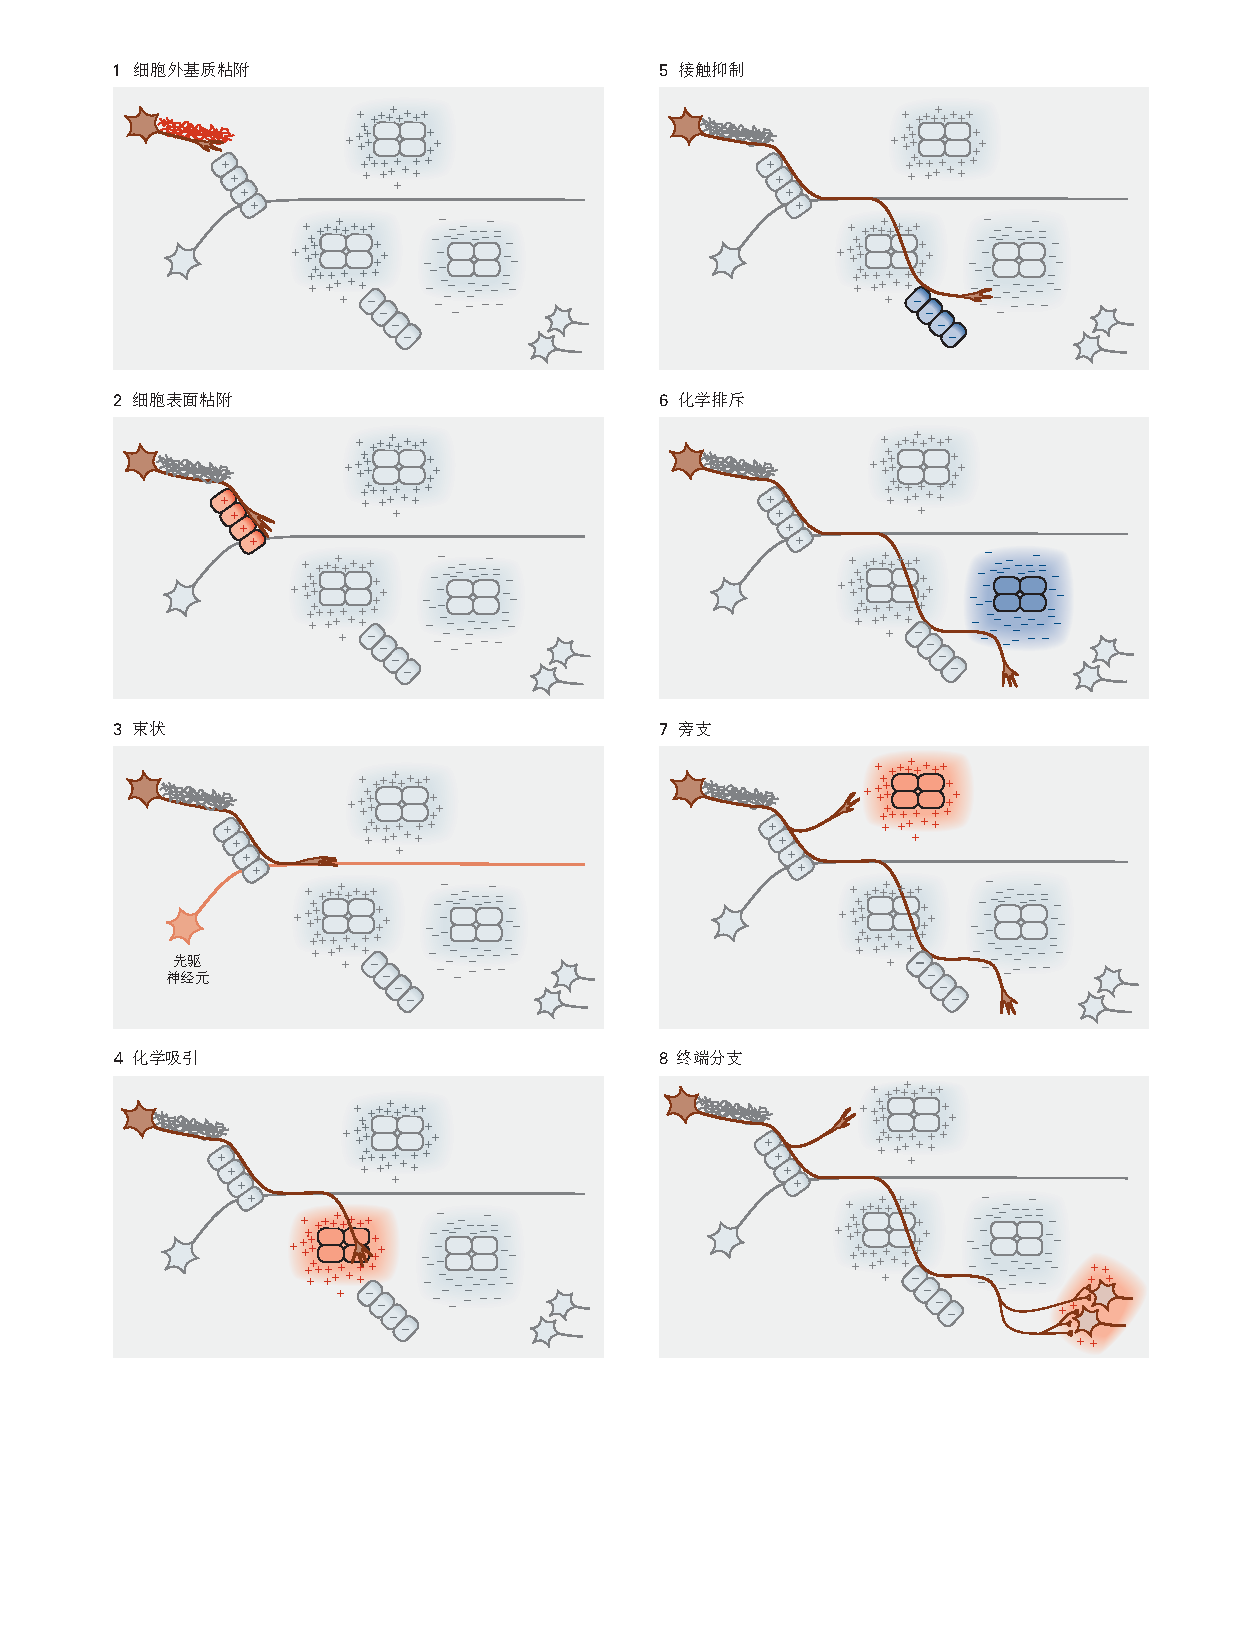
\includegraphics[width=0.95\linewidth]{chap47/fig_47_10}
	\caption{细胞外线索使用多种机制来引导生长锥。 轴突可以与细胞外基质中的生长促进分子相互作用 (1)。 它可以与神经细胞上的粘附细胞表面分子相互作用 (2)。 生长中的轴突会遇到来自“先驱”神经元的另一个轴突并沿着它移动,这一过程称为肌束震颤 (3)。 可溶性化学信号可以将生长的轴突吸引到其细胞源 (4)。 表达细胞表面排斥信号的中间靶细胞可导致轴突转向 (5)。 可溶性化学信号可以排斥生长中的轴突 (6)。 细胞外信号还导致从轴突轴 (7) 形成侧支或生长轴突 (8) 的分支。}
	\label{fig:47_10}
\end{figure}


这种轨迹的差异反映了来自鼻侧和颞侧视网膜的轴突对中线交叉细胞呈现的引导线索的不同反应。
一些视网膜轴突接触并穿过视交叉细胞,而另一些则被这些细胞抑制并偏转,从而留在同侧。
交叉细胞呈现的关键分子之一是 ephrin-B 家族的膜结合驱虫剂(图 \ref{fig:47_13}B),它也出现在视网膜神经节细胞轴突导向的后续步骤中。


向同侧投射的颞叶视网膜轴突的比例因物种而异:低等脊椎动物中很少,啮齿类动物中有一些,而人类中有很多。
这些差异反映了眼睛的位置。
在许多动物中,眼睛指向两侧并监视视觉世界的不同部分,因此不需要合并来自两只眼睛的信息。
在人类中,双眼向前看并采样视觉世界中大部分重叠的区域,因此视觉输入的协调至关重要。


穿过视交叉后,视网膜轴突沿着间脑的腹侧表面聚集在视束中。
然后轴突在不同的点离开管道。
在大多数脊椎动物物种中,中脑顶盖(在哺乳动物中称为上丘)是视网膜轴突的主要目标,但少数轴突投射到丘脑的外侧膝状体核。
然而,在人类中,大多数轴突投射到外侧膝状体,相当多的轴突投射到丘,小部分投射到枕核、视交叉上核和顶盖前核。
在这些目标中,不同的视网膜轴突投射到不同的区域。
正如 Sperry 所展示的,视网膜轴突在顶盖表面形成了精确的视网膜专题图。
类似的地图在其他由视网膜轴突支配的区域形成,例如外侧膝状体核。


到达顶盖内的适当位置后,视网膜轴突需要找到合适的突触伙伴。
为了完成他们旅程的最后一站,视网膜轴突转向并潜入顶盖神经细胞(图 \ref{fig:47_12}),沿着放射状神经胶质细胞表面下降(或者,在哺乳动物中,上升),这为放射状轴突生长提供了支架。
虽然放射状神经胶质细胞跨越神经上皮的整个范围,但每个视网膜轴突将其突触末端限制在单层。
许多突触后细胞的树突延伸穿过多层并沿其整个长度形成突触,但视网膜输入仅限于目标神经元树突树的一小部分。
这些组织特征意味着特定于层的线索会阻止轴突伸长并触发树枝化。


因此,长距离轴突导航的问题通过将旅程分成短段来解决,在这些短段中,中间目标引导轴突沿着路径到达最终目标。
一些中间目标,例如视交叉,是轴突发散的“决策”区域。


依靠中间目标是解决远距离轴突导航问题的有效方法,但不是唯一的方法。
在某些情况下,当胚胎较小且要覆盖的距离较短时,第一个轴突会到达它们的目标。
这些“先锋”轴突沿途对嵌入细胞或细胞外基质的分子信号作出反应。
第一个离开视网膜的轴突属于这一类。
较晚出现的轴突,当距离较长且障碍物较多时,可以跟随先驱到达它们的目标。
另一种引导机制是分子梯度。
事实上,正如我们将看到的,顶盖中细胞表面分子的梯度会告知轴突其正确的终止区。



\subsection{Ephrins 的梯度在大脑中提供抑制信号}

到目前为止,我们已经了解了视网膜轴突如何通过响应一系列离散的方向线索来到达顶盖。
然而,生长过程中的这些选择并不能解释 Sperry 对顶盖视网膜专题图的分析所暗示的平滑分级连接。
对假设的“地图分子”的探索成为发育神经生物学家的主要关注点,因此我们对其进行了一些详细描述。


随着生物测定的发展,对这些分子的探索取得了重大突破,其中来自视网膜特定部分的外植体被放置在顶盖膜碎片的基质上。
膜碎片取自顶盖的明确前后部分,并排列成交替的条纹。 
发现来自颞侧(后侧)半视网膜的轴突优先生长在来自前顶盖的膜上,这种偏好类似于体内表现出来的偏好(图 \ref{fig:47_14})。
发现这种偏好是由于后膜中存在抑制因子而不是前膜中有吸引力或粘附物质引起的。
这一观察是最早证明抑制或排斥物质在轴突引导中的作用的观察之一。


\begin{figure}[htbp]
	\centering
	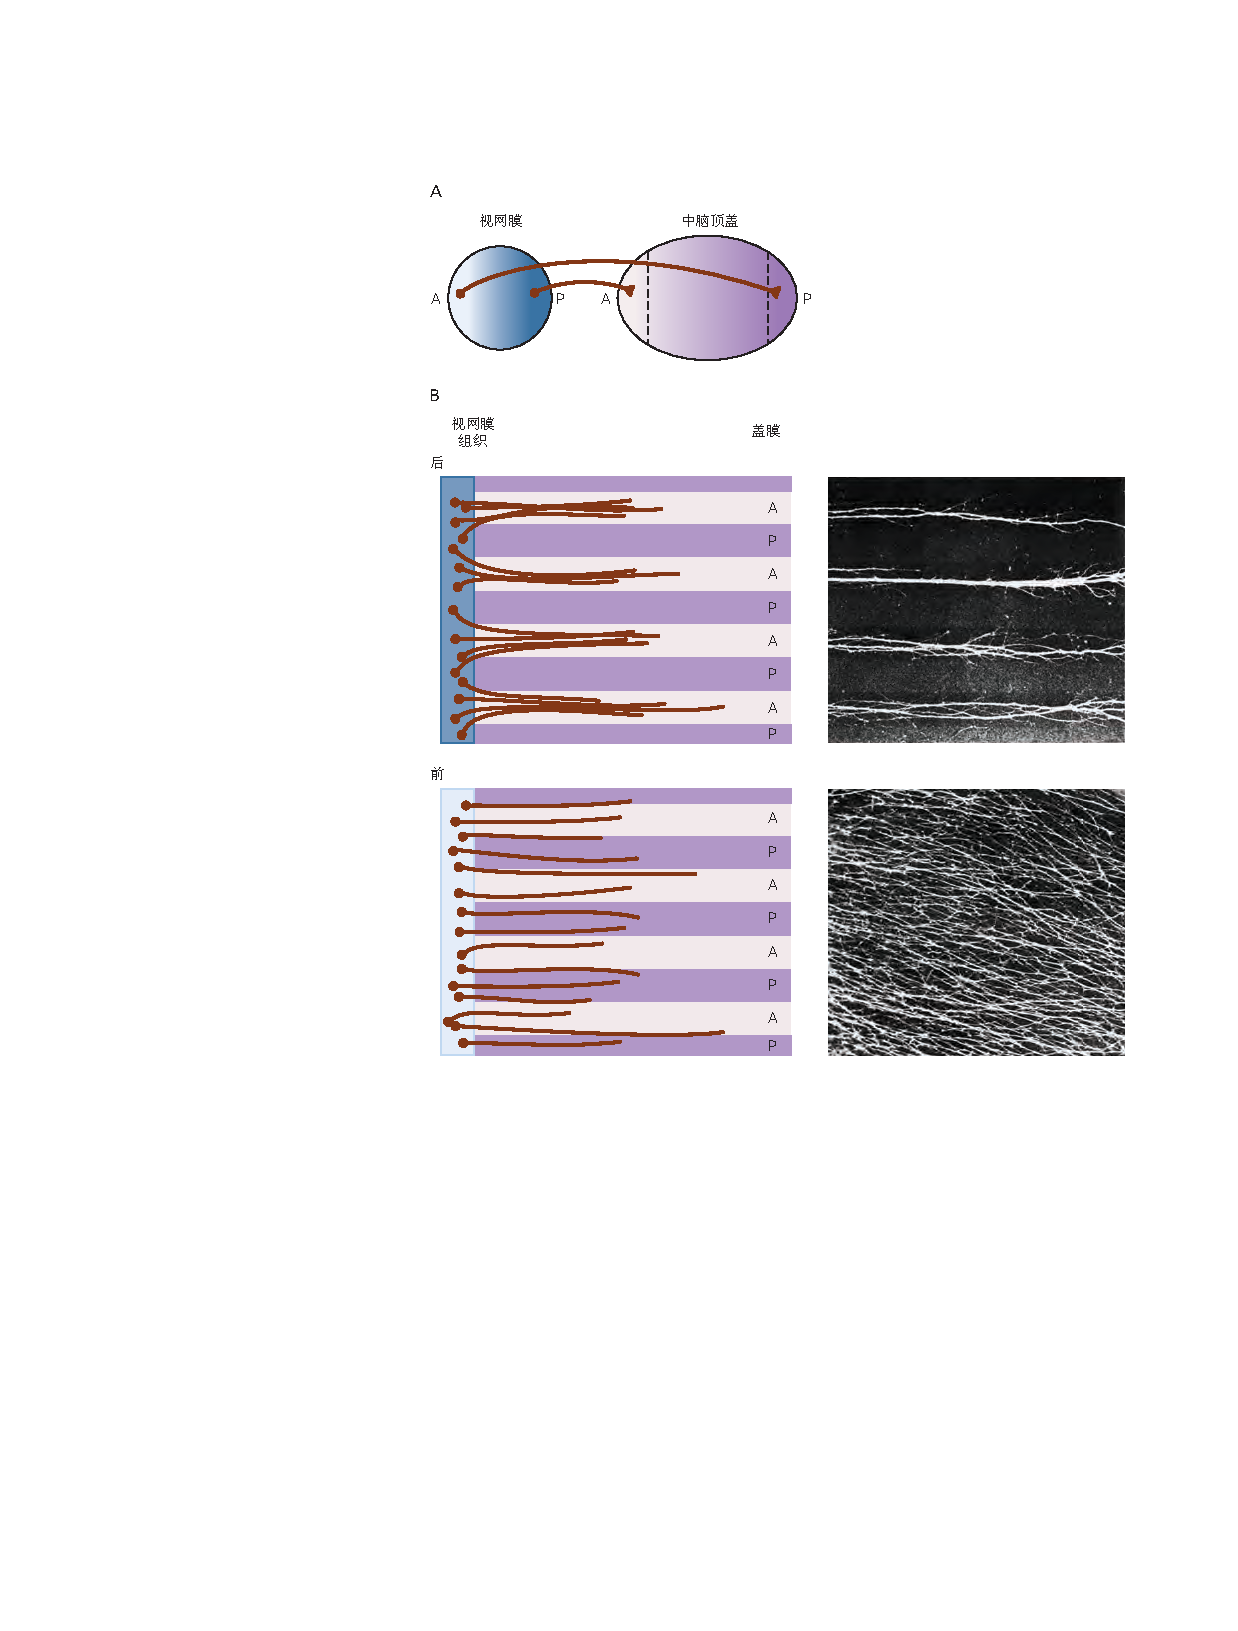
\includegraphics[width=0.75\linewidth]{chap47/fig_47_14}
	\caption{驱虫信号在体外指导视网膜轴突的发育。 A. 来自后部(颞侧)半视网膜的视网膜神经节轴突投射到前部发育中的顶盖中。 相反,来自前(鼻)半视网膜的轴突投射到后顶盖。 B. 膜碎片取自顶盖的特定前后部分,并排列成交替的条带。 来自后部视网膜外植体的轴突选择性地生长在前顶盖的碎片上。 轴突在前膜上的优先生长是由后膜中的抑制信号引起的。 相反,来自前部视网膜的轴突生长在前后盖膜碎片上。 (缩写:A,前部;P,后部。)(经许可改编自 Walter、Henke-Fahle 和 Bonhoeffer 1987。)}
	\label{fig:47_14}
\end{figure}


这种条纹测定允许表征抑制线索,存在于后顶盖的膜中而不是前顶盖。
独立地,分子生物学家鉴定了一个受体酪氨酸激酶家族,即 Eph 激酶,以及一个大家族的膜相关配体,肝配蛋白。
受体和配体都分为 A 和 B 亚族。
ephrin-A 蛋白结合并激活 EphA 激酶;
相反,ephrin-B 蛋白结合并激活 EphB 激酶(图 \ref{fig:47_11}C)。


\begin{figure}[htbp]
	\centering
	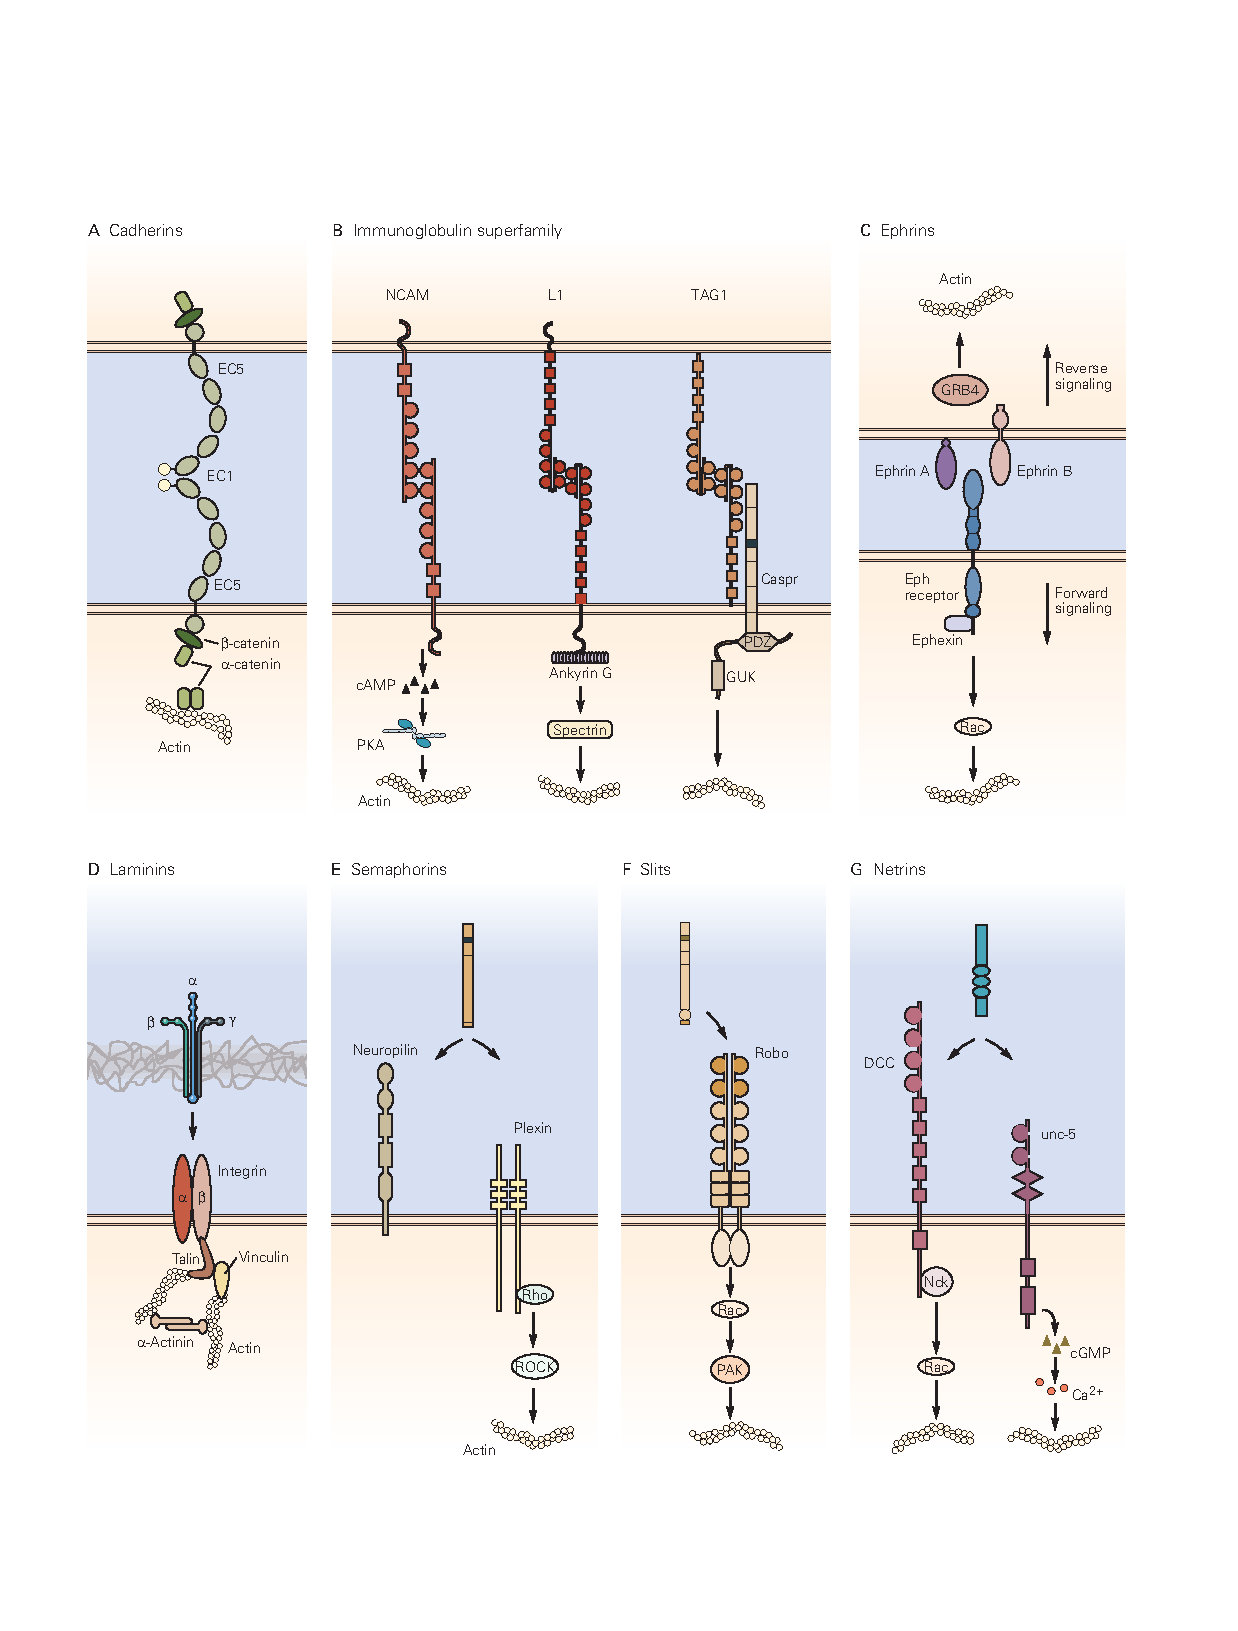
\includegraphics[width=0.95\linewidth]{chap47/fig_47_11}
	\caption{}
	\label{fig:47_11}
\end{figure}


当 tectal 抑制线索被确定为 ephrin-A5 时,这两条研究线汇聚在一起。
我们现在知道,Eph 激酶和肝配蛋白在神经和非神经组织中发挥多种功能,并且每一类蛋白质都可以作为配体或受体,具体取决于细胞环境。
在发育中的神经系统中,这些蛋白质构成了主要的驱避信号组。


Ephrin-Eph 相互作用在很大程度上解释了顶盖中视网膜专题图的形成。
顶盖中肝配蛋白-A2 和肝配蛋白-A5 的水平以及视网膜中 Eph 受体的水平沿前后轴分级。
这些梯度沿同一方向运行。
Ephrin-A 浓度在顶盖中从后高到前低,而 Eph A 浓度在视网膜中从后高到前低(图 \ref{fig:47_15}A)。
这种反梯度至少部分地解释了地形图。
来自具有高水平 EphA 受体的后视网膜神经节细胞的轴突被后顶盖中高水平的肾上腺素 A 排斥得最强烈,因此被限制在前顶盖。
来自前部视网膜的不太敏感的轴突能够进一步穿透到顶盖的后部区域。
因此肝配蛋白-A2 和肝配蛋白-A5 是 Sperry 假定类型的化学特异性因子的有力候选者。


\begin{figure}[htbp]
	\centering
	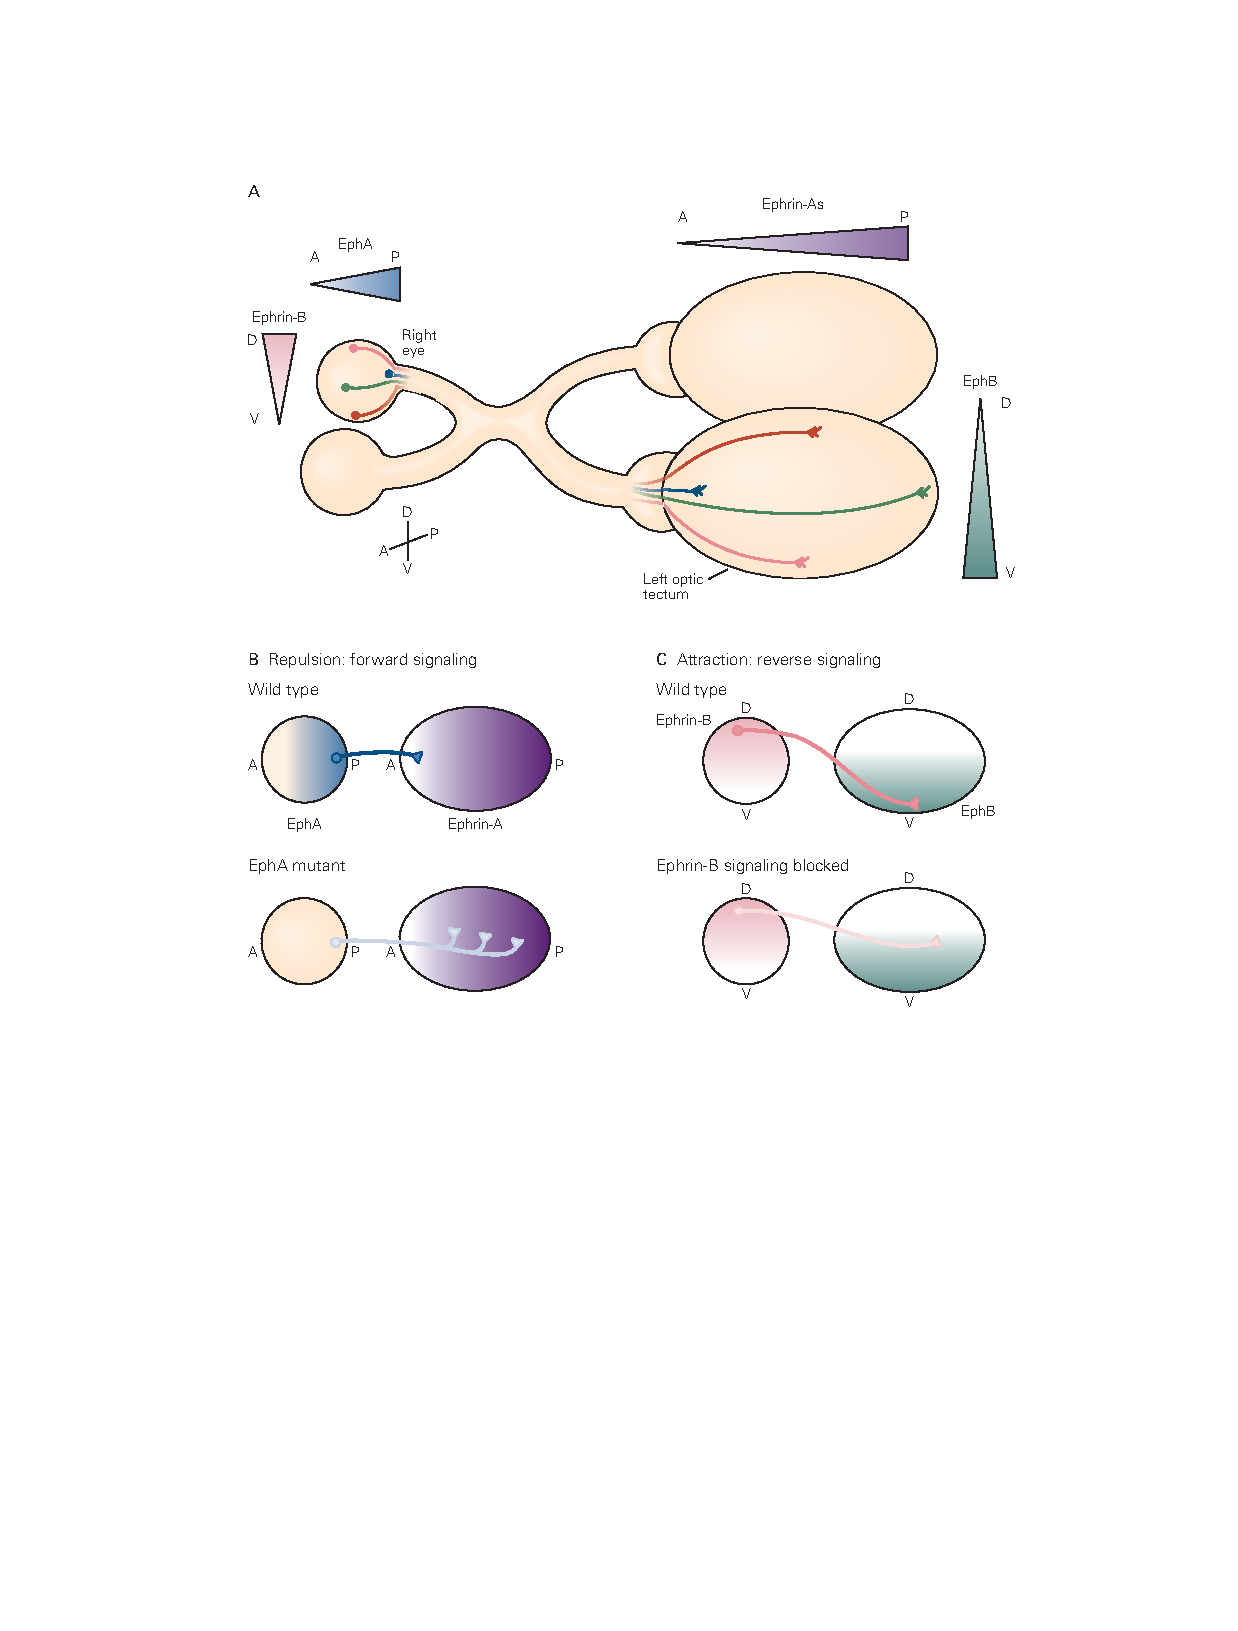
\includegraphics[width=0.8\linewidth]{chap47/fig_47_15}
	\caption{体内视网膜专题图的形成取决于 ephrin-Eph 激酶信号。 A. 在视网膜中,EphA 受体以前后 (A-P) 梯度表达,ephrin-B 以背腹 (D-V) 梯度表达。 在顶盖中,ephrin-A 受体呈前后梯度分布,EphB 呈背腹梯度分布。 B. EphA 在源自后部(颞部)视网膜神经元的视网膜轴突中的表达通过避免 ephrin-A 蛋白将轴突生长引导至前顶盖。 在 EphA 突变小鼠中,后视网膜轴突能够投射到顶盖内更靠后的区域。 C. EphB 信号将背侧视网膜轴突投射到腹侧顶盖。 用可溶性 EphB 蛋白阻断 ephrin-B 信号传导会导致背轴突投射到顶盖内异常的背侧区域。}
	\label{fig:47_15}
\end{figure}


肝配蛋白和 Eph 激酶相互作用在视网膜专题图形成中的关键作用已在体内得到证实。
ephrin-A2 在发育中的鸡胚视顶盖中的过度表达在头顶盖中生成异常富含 ephrin-A2 的小块细胞。
通常避开富含肝配蛋白的尾顶盖的颞叶视网膜轴突也避开了头顶盖中的这些斑块,并且它们终止于异常位置。
相比之下,通常向尾顶盖生长的鼻部视网膜轴突不会因遇到过量的 ephrin-A 而受到干扰。


相反,在相关 ephA 或 ephrin-A 基因发生靶向突变的小鼠中,一些后部视网膜轴突终止于不适当的后顶盖区域(图 \ref{fig:47_15}B)。
自然表达低水平 EphA 蛋白的前视网膜轴突在这些突变体中正常投射。
在缺乏两种 ephrin-A 蛋白的小鼠中,这些缺陷比任何一种突变体都更严重。
因此,ephrin-A 与 EphA 受体的相互作用对于靶向顶盖中的视网膜轴突至关重要。
这些 ephrin/EphA 对具有 Sperry 预测的识别分子的特性,这些特性是沿着顶盖的前后轴进行地形图绘制所必需的。


当然,视网膜图也有背腹轴。
Ephrin/EphB 对参与沿此轴建立秩序。
正如 ephrin-A 和 EphA 沿前后轴分级,ephrin-B 和 EphB 沿背腹轴分级,ephrin-B 和 EphB 水平的操纵影响背腹映射(图 \ref{fig:47_15}C)。
因此,在简单的层面上,视网膜专题图排列在直角坐标系中,ephrin-A/EphA 和 ephrin-B/EphB 分别标记前后轴和背腹轴。


尽管这种简单的观点令人满意,但现实情况更为复杂。 首先,EphB 激酶在顶盖和视网膜中表达,肝配蛋白-A 在视网膜和顶盖中表达。
因此,可能涉及所谓的“顺式”相互作用(Eph 和肝配蛋白在同一细胞上)以及“反式”相互作用(Eph 在生长锥上,肝配蛋白在靶细胞上)。
其次,配体和受体都存在于光学通路的多个点上,并发挥着多重作用。
正如我们所见,ephrin-B/EphB 相互作用不仅影响背腹映射,还影响轴突在视交叉处穿过对侧的决定。
最后,在开发视觉回路时,更精确的视网膜输入空间映射受神经活动模式的调节,这将在接下来的两章中讨论。
尽管如此,我们现在已经大致了解了从眼睛到大脑的地形投射的初始形成的分子策略。



\section{一些脊髓神经元的轴突被引导穿过中线}

中枢神经系统的基本特征之一是需要协调身体两侧的活动。
为了完成这项任务,某些轴突需要投射到另一侧。


我们已经看到一个轴突在视交叉中交叉的例子。
另一个被详细研究过的例子是连合神经元的轴突交叉,这些神经元将感觉信息从脊髓传递到脊髓腹侧中线穿过底板的大脑。
交叉后,轴突突然转向并向大脑生长。
这个简单的轨迹提出了几个问题。
这些轴突如何到达腹侧中线?
它们如何穿过中线,以及在穿过后,它们如何忽略另一侧的轴突用来到达中线的线索?
换句话说,为什么它们转向大脑而不是返回?



\subsection{Netrins 直接开发跨中线的连合轴突}

许多将轴突发送到腹侧中线的神经元是在脊髓的后半部分产生的。
这些轴突的首要任务是到达腹侧中线。
Ramón y Cajal 考虑了目标发出的趋化因子可能吸引轴突的可能性,但这个想法沉睡了将近一个世纪。
我们现在知道这些因素确实存在,其中之一,蛋白质 netrin-1,由底板细胞以及沿腹侧中线的祖细胞表达。
当在培养物中出现时,netrin 吸引连合轴突;
当小鼠被剥夺 netrin-1 功能时,轴突无法到达底板(图 \ref{fig:47_16})。
它可以作为分泌因子(趋化性)和膜引导分子(趋触性)来引导连合神经元的轴突到达底板。


\begin{figure}[htbp]
	\centering
	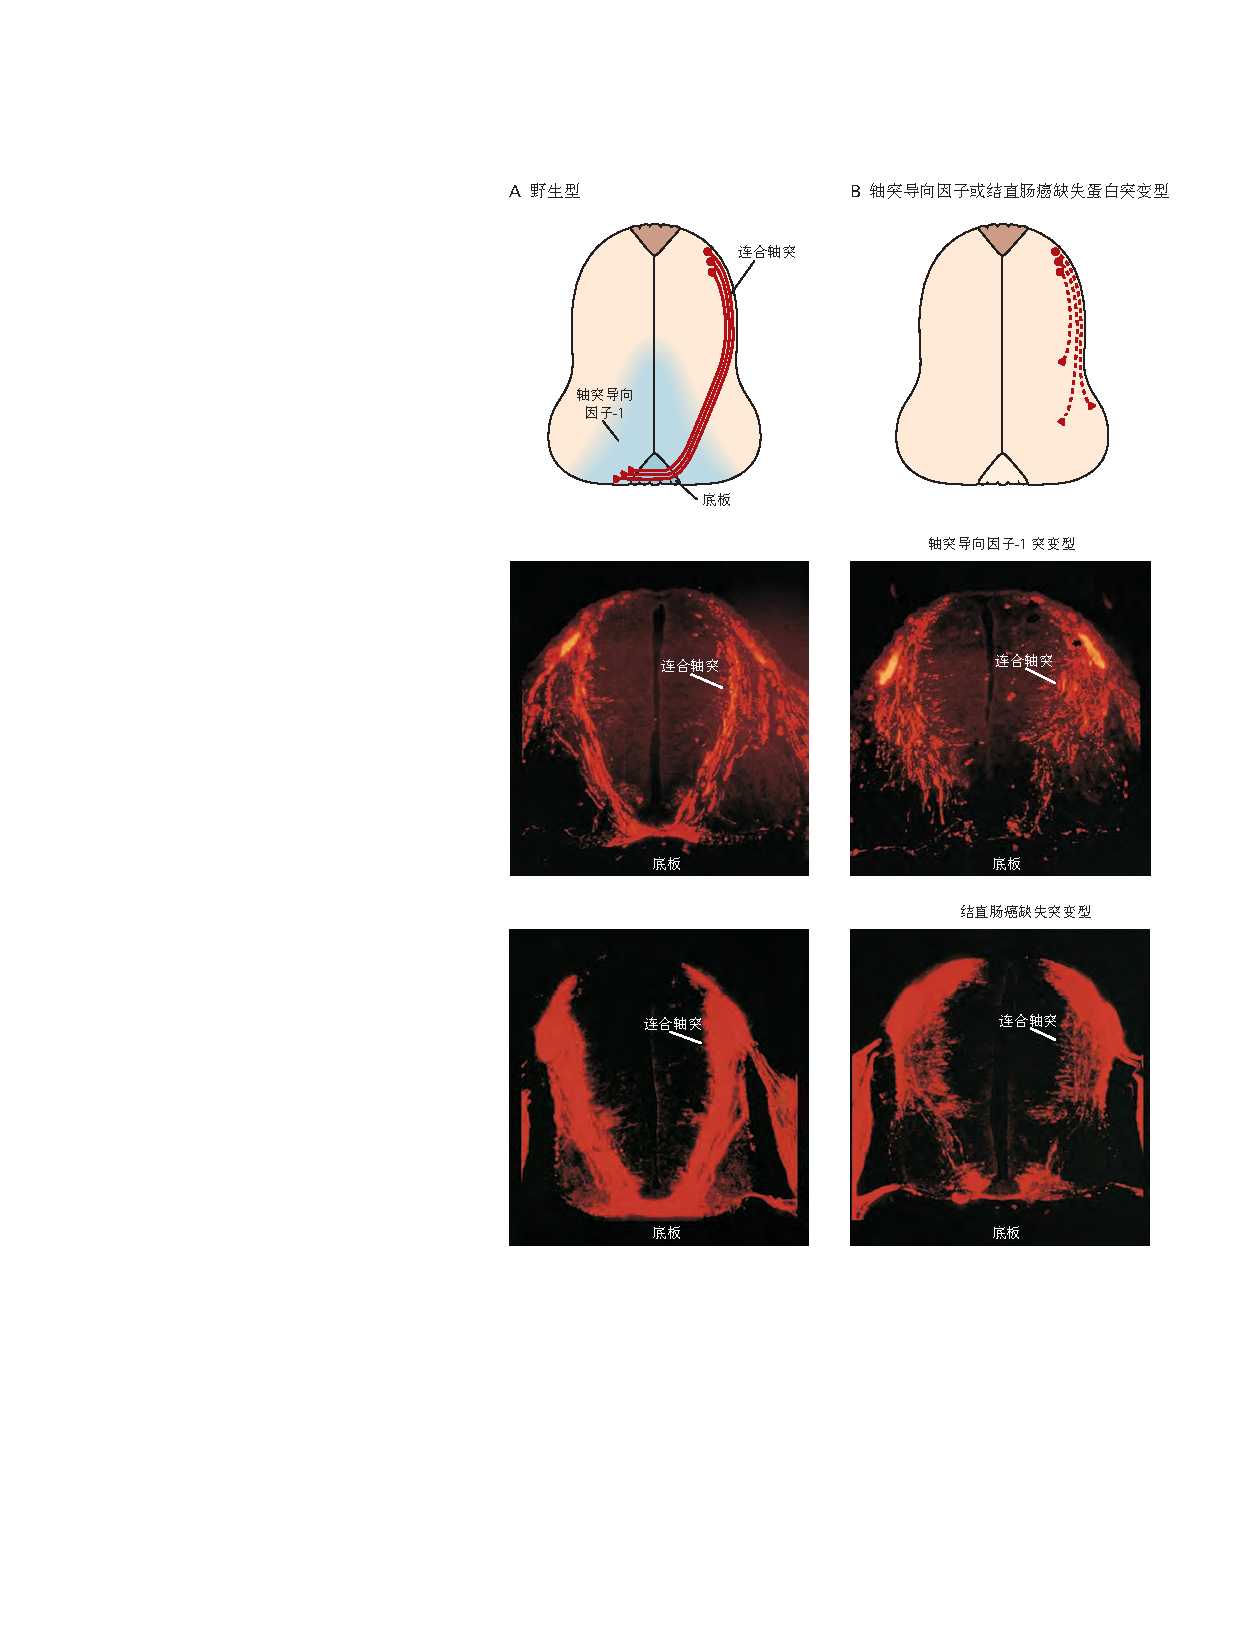
\includegraphics[width=0.65\linewidth]{chap47/fig_47_16}
	\caption{Netrin 信号将脊髓连合神经元的轴突吸引到底板上。 (显微照片经许可转载自 Marc Tessier-Lavigne。) A. Netrin-1 由底板细胞和腹侧神经祖细胞产生。 它将连合神经元的轴突吸引到脊髓腹侧中线的底板 (FP)。 B. 当结直肠癌 (DCC) 蛋白中的 netrin 或缺失蛋白被消除时,大多数连合轴突无法到达底板。}
	\label{fig:47_16}
\end{figure}


netrin 蛋白在结构上与 unc-6 的蛋白质产物相关,unc-6 是一种显示在线虫梭状芽孢杆菌中调节轴突导向的基因。
另外两个秀丽隐杆线虫基因 unc-5 和 unc-40 编码 unc-6 蛋白的受体。
脊椎动物 netrin 受体与 unc-5 和 unc-40 受体有关。
unc-5H 蛋白是 unc-5 的同系物,DCC(在结直肠癌中缺失)与 unc-40 相关(参见图 \ref{fig:47_11}G)。
这些受体是免疫球蛋白超家族的成员,它们的功能在整个动物进化过程中都非常保守(图 \ref{fig:47_17})。
这种保护支持使用简单且遗传上可获得的无脊椎动物来揭示发育的复杂性。
在任何领域,这种方法都比在轴突导向分析中更有成效。
影响这一过程的数十个基因首先在果蝇和线虫中被鉴定和克隆,然后被证明在哺乳动物中发挥重要和相关的作用。


\begin{figure}[htbp]
	\centering
	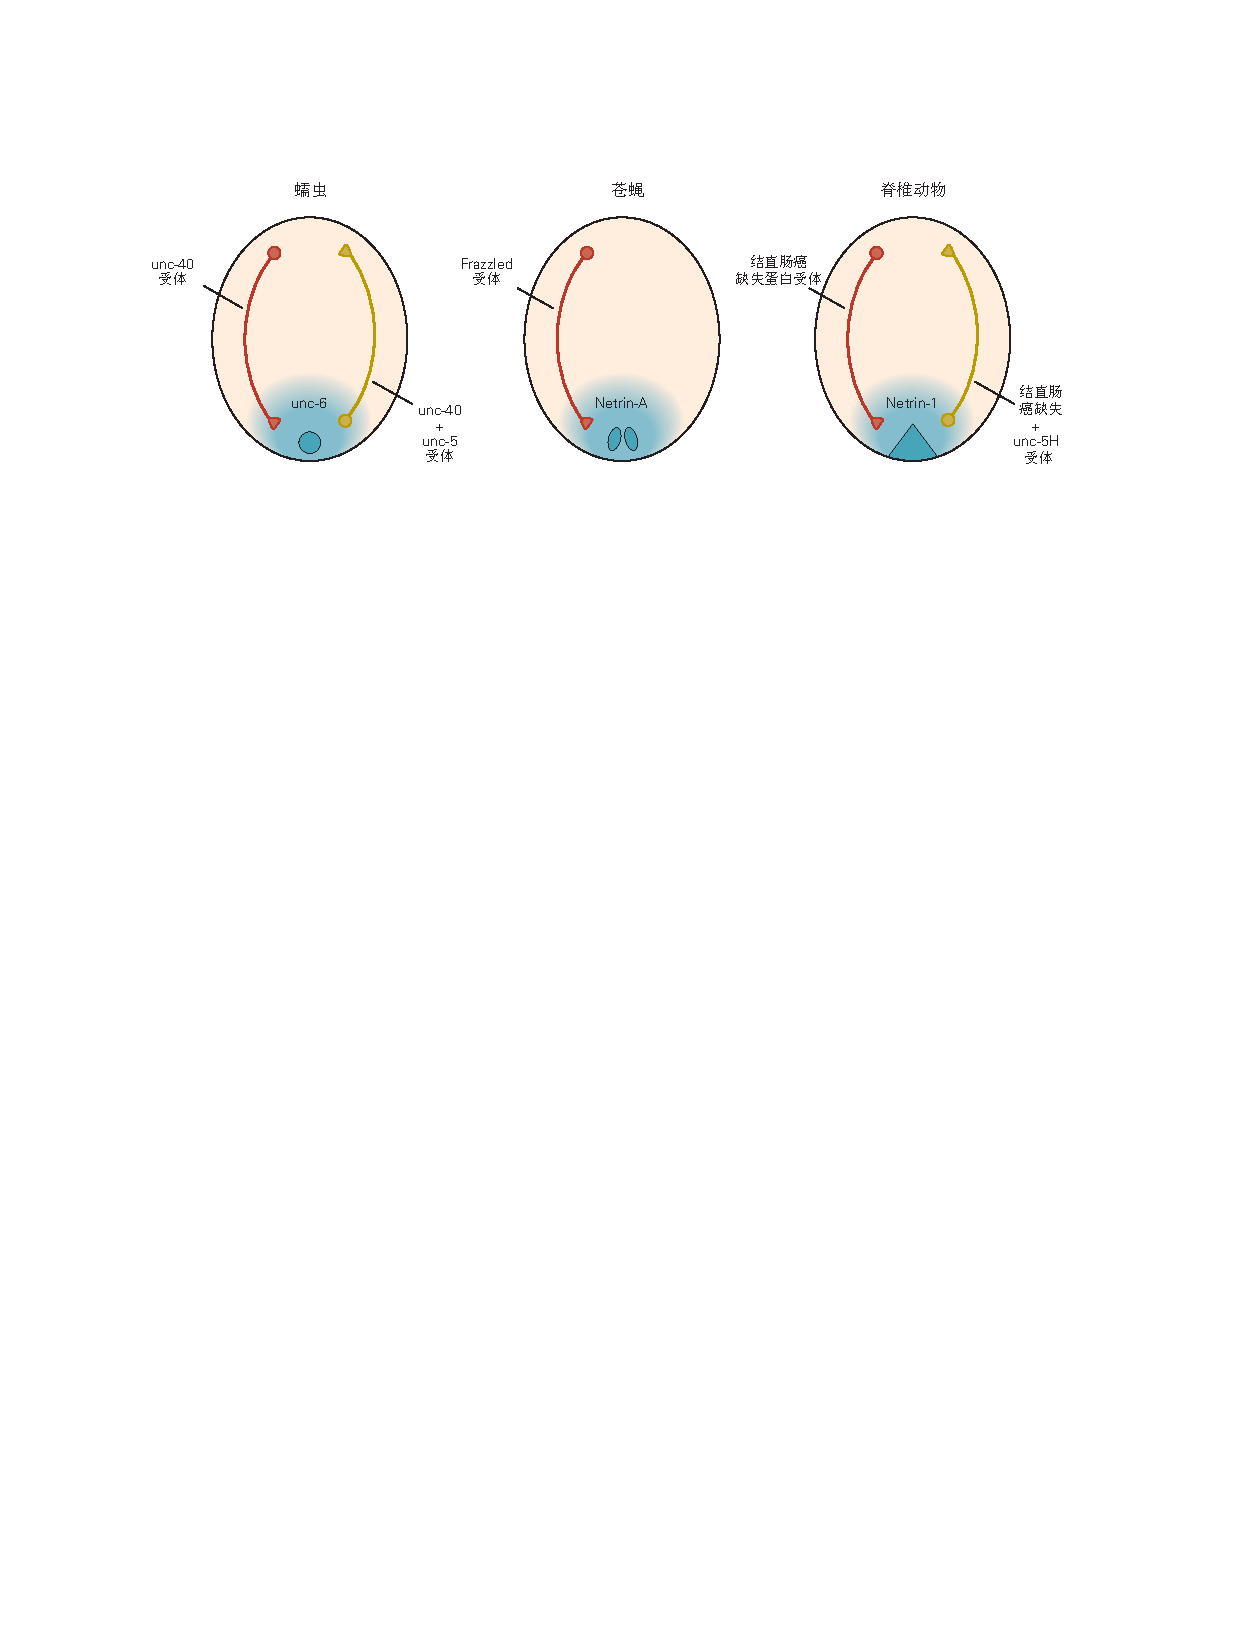
\includegraphics[width=0.8\linewidth]{chap47/fig_47_17}
	\caption{netrins 的表达和活性在整个进化过程中一直保持不变。 Netrins 由蠕虫、果蝇和脊椎动物的腹侧中线细胞分泌,并与沿背腹轴迁移或延伸的细胞或轴突上的受体相互作用。 结直肠癌 (DCC)(脊椎动物)中的 netrin 受体 unc-40(蠕虫)、frazzled(苍蝇)和缺失介导 netrin 的引诱活性,而 unc-5 类受体介导其驱避活性。}
	\label{fig:47_17}
\end{figure}


\subsection{趋化因子和趋化因子影响中线}

其他信号系统与 netrin 一起工作以引导连合轴突。 一组由骨形态发生蛋白组成,由屋顶板分泌。
它们充当驱虫剂,在它们开始它们的旅程时将连合轴突引导到腹侧。
来自底板的其他因素,例如最初参与脊髓模式化的刺猬蛋白(第 \ref{chap:chap45} 章),可能在后期与 netrins 合作,作为轴突引诱剂。


一旦连合轴突到达中线,它们就会发现自己暴露在可用的最高水平的 netrin-1 和 sonic hedgehog 中。
然而,这种富含 netrin 的环境并不能无限期地将轴突保持在中线。
相反,它们穿过脊髓的另一侧,即使它们的对侧对应物正在向上导航 netrin 趋化梯度。


这种令人费解的行为可以解释为生长锥由于暴露于底板信号而改变了它们对吸引和排斥信号的响应。
这个开关说明了参与轴突引导的中间目标的一个重要特性。
中间目标呈现的因素不仅引导轴突的生长,而且改变生长锥的敏感性,为下一阶段的旅程做好准备。


一旦轴突到达底板,它们就会对 Slit 敏感,Slit 是底板细胞分泌的化学排斥信号(图 \ref{fig:47_18})。
在连合轴突到达底板之前,作为 Slit 受体的 Robo 蛋白通过相关蛋白 Rig-1 的表达保持非活性。
当轴突到达底板时,其表面的 Rig-1 水平下降,释放 Robo 活动并导致轴突对 Slit 的排斥作用做出反应。
这种驱避作用推动生长锥沿着狭缝梯度进入脊髓的对侧。 此外,激活的 Robo 与 DCC 形成复合物,使这些 Netrin 受体无法对其配体作出反应。
生长锥对底板吸引特性的敏感性降低有助于解释底板信号对轴突的瞬态影响。


\begin{figure}[htbp]
	\centering
	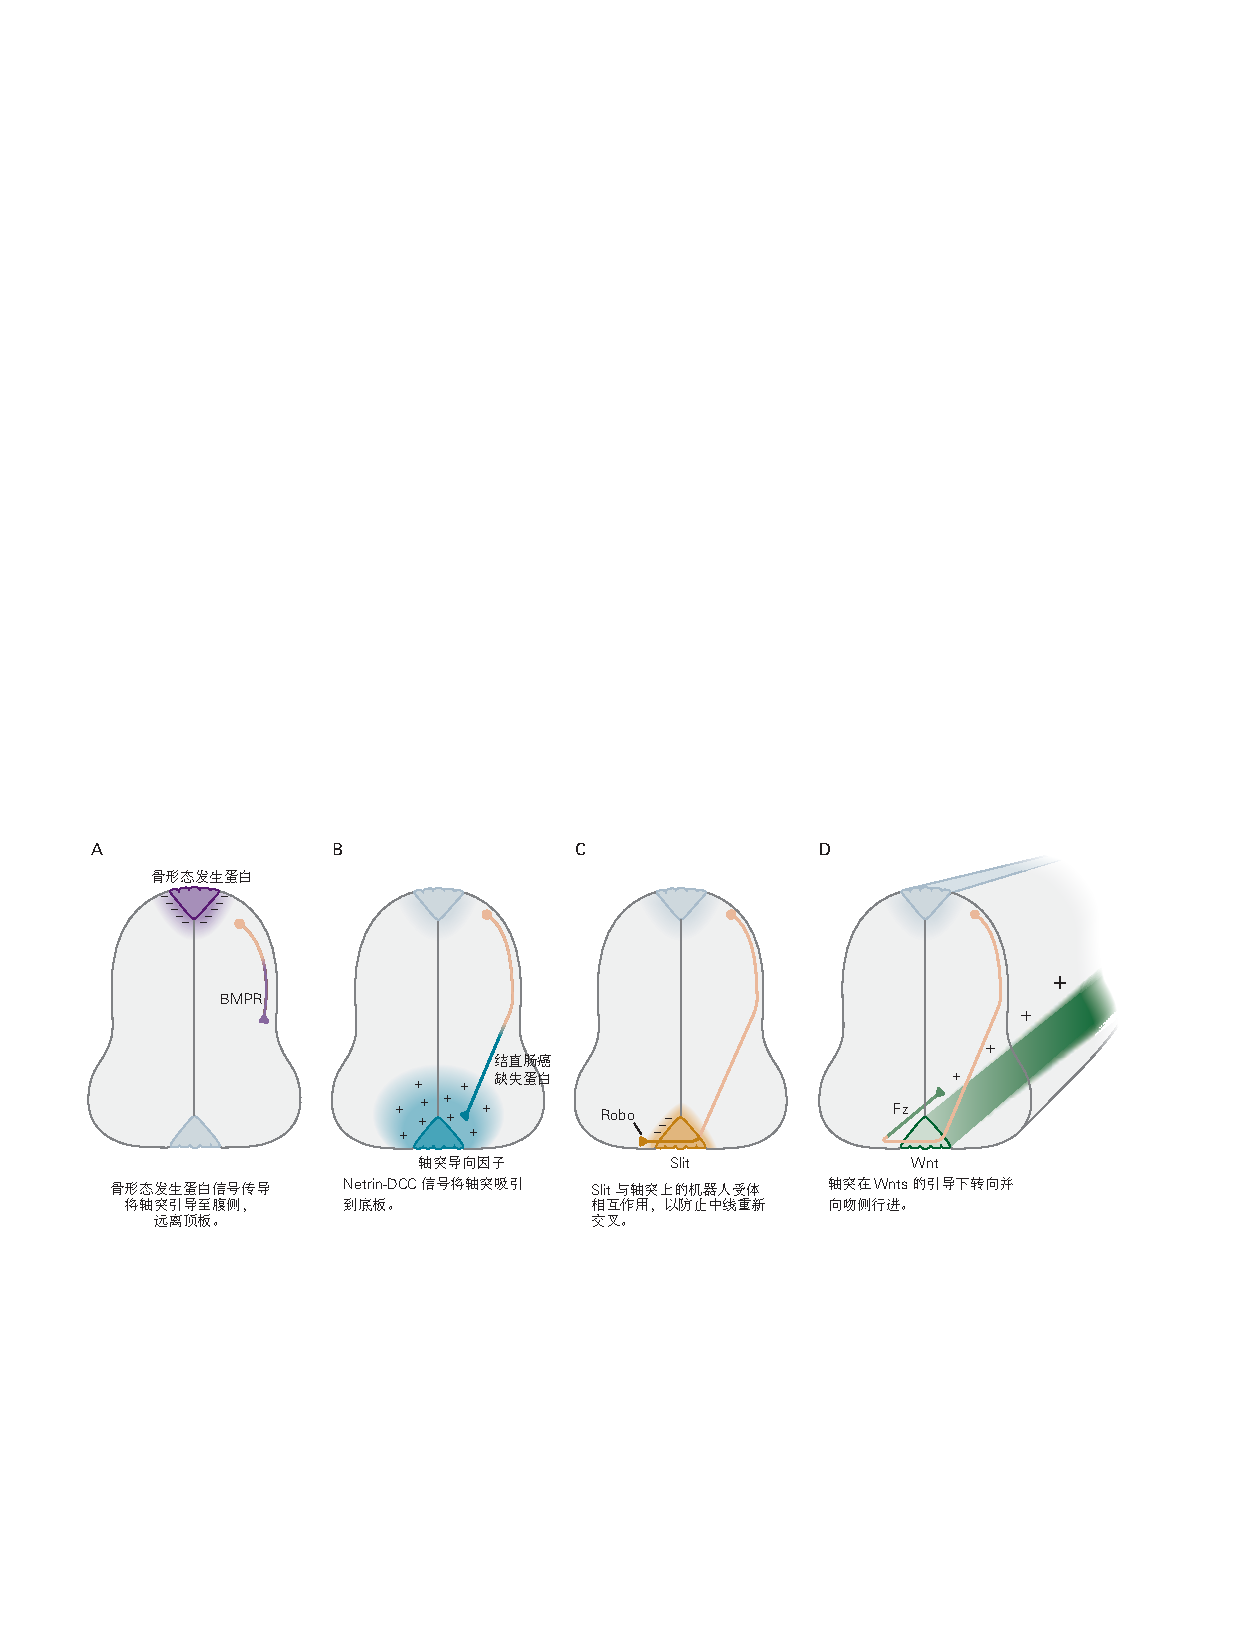
\includegraphics[width=0.95\linewidth]{chap47/fig_47_18}
	\caption{顶板和底板细胞表达的指导线索指导发育中的脊髓中的连合轴突。 A. 屋顶板细胞分泌的骨形态发生蛋白 (BMP) 与连合轴突上的 BMP 受体 (BMPR) 相互作用,以引导轴突远离屋顶板。 B. 由底板细胞表达的 Netrin 吸引在结直肠癌 (DCC) 中缺失的表达连合轴突到脊髓的腹侧中线。 Sonic hedgehog 也与连合轴突的腹侧引导有关。 C. 底板细胞分泌的 Slit 蛋白与连合轴突上的 Robo 受体相互作用,以防止这些轴突再次穿过中线。 在穿越之前,但不是之后,除了 robo1 和 robo2 之外,连合轴突还表达 robo3 (Rig-1)。 Rig-1 蛋白使 Robo 受体失活,防止轴突在靠近腹侧中线时对 Slits 的驱避作用做出反应。 D. 连合轴突穿过中线后,底板细胞分泌的 Wnt 蛋白以 rostrocaudal 梯度分布,与连合轴突上的卷曲 (Fz) 蛋白相互作用,将轴突引向大脑。}
	\label{fig:47_18}
\end{figure}


最后,一旦轴突离开底板,它们就会转向大脑中最终的突触目标。
底板细胞表达的 Wnt 蛋白的尾端梯度似乎在腹侧中线处引导轴突向嘴侧生长(图 \ref{fig:47_18}D)。
因此,不同的线索在其整体轨迹的不同阶段指导连合轴突。
同样的过程可能会在数百甚至数千类神经元中进行,以建立成熟的大脑连接模式。



\section{要点}

1. 随着神经元的延伸过程,一个通常变成轴突,其他变成树突。
这个过程称为极化。
这两种类型的过程在结构和分子结构以及功能上有所不同。 


2. 细胞类型在其树突的形状、大小和分支模式方面存在显着差异。
特定类型的树突特征既来自类型间转录程序的内在差异,也来自对发育中的树突的外在影响。


3. 树突之间的相互作用对于树突图案化至关重要。
单个细胞的树突之间的排斥相互作用(称为自我回避的过程)导致区域的均匀覆盖,具有最小的间隙或团块。
相邻细胞的树突之间的排斥作用(称为平铺的过程)可最大限度地减少树突区域的重叠。
在某些情况下,树突会避开其自身神经元的其他树突,但会与名义上相同的相邻细胞的树突相互作用。
这个过程称为自我/非自我歧视。


4. 轴突顶端的生长锥作为感觉和运动元件,引导轴突到达目的地。
生长锥的细胞骨架元素,包括肌动蛋白和肌球蛋白,促进生长。


5. 生长锥上的受体识别并结合轴突延伸所经过的环境中的配体,从而引导生长。
这些相互作用导致它们的第二信使的产生,这些第二信使介导生长、生长锥的转动和停止以及轴突的分支。


6. 一些生长锥包含蛋白质合成机器,包括信使 RNA。
在这些情况下,受体可以促进介导生长或转变的特定蛋白质的局部合成。


7. 配体-受体对包括几个关键的分子家族,包括钙粘蛋白、Slits 及其 Robo 受体、脑信号蛋白及其神经丛蛋白受体,以及肝配蛋白及其 Eph 激酶受体。


8. 轴突向远处目标的生长被分解成离散的较短步骤。 在每一步中,相邻结构表面的分子或由相邻结构分泌的分子都会引导轴突。
它们还可以导致生长锥的受体补充发生变化,使其能够在后续阶段对不同的线索集做出反应。


9. Roger Sperry 提出了一个化学特异性假说来解释轴突从视网膜不同部位到视顶盖(上丘)不同部位的特定生长,形成有序的视网膜专题图。
肝配蛋白及其受体 Eph 激酶是指导图谱形成的关键分子。
它们沿着视网膜和顶盖的表达分级,并且在很大程度上通过将轴突从不正确的位置排斥而不是将它们吸引到正确的位置来起作用。


10. 吸引分子和排斥分子都引导轴突穿过中线结构,这一过程称为交叉。
进化上保守的信号包括 Slits、netrins 和 Wnts。
编码这些配体和受体的基因突变可导致发育性神经系统疾病。

